\documentclass[aspectratio=169,11pt]{beamer}

% ================================================================
% Day 3 Morning: NUFFT, Fast Ewald Summation, and the DMK Framework
% Fast Algorithms and Integral Equation Methods -- AMSS Summer Course
% Target: graduate students / young researchers. Two hours (~110 slides),
% with a 10 minute break after the Ewald/ESP block.
% ================================================================

\IfFileExists{beamerthemeCCM.sty}{%
  \usetheme{CCM}
}{%
  \usetheme{default}
  \definecolor{CCMorange}{HTML}{F6862D}
  \definecolor{SFdark}{HTML}{1D2954}
  \definecolor{mygray}{HTML}{8F8F8F}
  \setbeamertemplate{navigation symbols}{}
  \setbeamertemplate{footline}[frame number]
  \setbeamersize{text margin left=0.25in,text margin right=0.25in}
  \setbeamercolor{title}{fg=CCMorange}
  \setbeamercolor{frametitle}{fg=CCMorange,bg=white}
  \setbeamercolor{item}{fg=CCMorange}
  \setbeamercolor{block title}{fg=black,bg=CCMorange!30}
  \setbeamercolor{block body}{fg=black,bg=black!3}
  \setbeamercolor{section in toc}{fg=SFdark}
}

\usepackage{amsmath,amssymb,mathtools}
\usepackage{bm}
\usepackage{booktabs}
\usepackage{graphicx}
\usepackage{times}
\usepackage{tikz}
\usetikzlibrary{arrows.meta,calc,decorations.pathreplacing,positioning,backgrounds,fit}

\graphicspath{{day3_morning_figures/}{./}}

% ---- math shorthands ----
\newcommand{\R}{\mathbb{R}}
\newcommand{\C}{\mathbb{C}}
\newcommand{\Z}{\mathbb{Z}}
\newcommand{\cO}{\mathcal{O}}
\newcommand{\cF}{\mathcal{F}}
\newcommand{\cD}{\mathcal{D}}
\newcommand{\cN}{\mathcal{N}}
\newcommand{\cR}{\mathcal{R}}
\newcommand{\dd}{\,\mathrm d}
\newcommand{\ii}{\mathrm i}
\newcommand{\x}{\bm{x}}
\newcommand{\y}{\bm{y}}
\newcommand{\kk}{\bm{k}}
\newcommand{\mm}{\bm{m}}
\newcommand{\nnn}{\bm{n}}
\newcommand{\rr}{\bm{r}}
\newcommand{\svec}{\bm{s}}
\newcommand{\cc}{\bm{c}}
% Shared operator notation for the AMSS FIEM talk slides.
% Change this one line to change the font for layer and volume potentials.
\newcommand{\FIEMopfont}[1]{\mathcal{#1}}

\newcommand{\Sop}{\FIEMopfont{S}}
\newcommand{\Dop}{\FIEMopfont{D}}
\newcommand{\Spop}{\Sop^{\prime}}
\newcommand{\Dpop}{\Dop^{\prime}}
\newcommand{\Vop}{\FIEMopfont{V}}
\newcommand{\Iop}{\FIEMopfont{I}}
\newcommand{\Kop}{\FIEMopfont{K}}
\newcommand{\KopT}{\Kop^{\prime}}
\newcommand{\Wop}{\FIEMopfont{W}}
\newcommand{\Aop}{\FIEMopfont{A}}
\newcommand{\Top}{\FIEMopfont{T}}

\newcommand{\hl}[1]{{\color{CCMorange}\textbf{#1}}}
\newcommand{\gray}[1]{{\color{mygray}#1}}
\DeclareMathOperator{\dist}{dist}
\DeclareMathOperator{\erf}{erf}
\DeclareMathOperator{\erfc}{erfc}
\DeclareMathOperator{\sinc}{sinc}

\setbeamertemplate{section in toc}[sections numbered]

\title{Day 3 Morning: NUFFT, Fast Ewald Summation, and the DMK Framework}
\subtitle{Dual-space formulations for fast summation and convolution}
\author{Fast Algorithms and Integral Equation Methods}
\institute{AMSS Summer Course \quad (Shidong Jiang)}
\date{July 2026}

\begin{document}

%================================================================
\begin{frame}
  \titlepage
\end{frame}

%================================================================
\begin{frame}{NUFFT, Ewald, and DMK roadmap}
\small
\begin{columns}[T,totalwidth=\textwidth]
\begin{column}{0.32\textwidth}
\textbf{Part I --- nonuniform FFT (NUFFT) \((\approx30\) min)}
\begin{itemize}\itemsep2pt
  \item The three nonuniform transforms.
  \item Spread \(\to\) FFT \(\to\) correct.
  \item Kernels and error analysis.
  \item Complexity; \texttt{finufft}.
\end{itemize}
\end{column}
\begin{column}{0.32\textwidth}
\textbf{Part II --- fast Ewald / ESP \((\approx20\) min)}
\begin{itemize}\itemsep2pt
  \item Periodic Coulomb sums.
  \item Ewald splitting; NUFFT acceleration of the reciprocal sum.
  \item ESP = Ewald summation with prolates.
\end{itemize}
\vspace{2mm}
\centerline{\hl{10 minute break}}
\end{column}
\begin{column}{0.32\textwidth}
\textbf{Part III --- dual-space multilevel kernel splitting (DMK) \((\approx50\) min)}
\begin{itemize}\itemsep2pt
  \item Multilevel kernel splitting.
  \item Dual-space representation.
  \item Diagonal translation, no global FFT.
  \item Adaptive \(\cO(N)\) algorithm.
\end{itemize}
\end{column}
\end{columns}

\vspace{3mm}
\begin{block}{How the three pieces relate}
NUFFT accelerates nonequispaced Fourier sums. Ewald splits the kernel once
into a short-range physical part and a smooth reciprocal-space part; the
reciprocal sum can be accelerated by FFT/NUFFT. DMK applies kernel splitting
on a hierarchy of levels.
\end{block}
\end{frame}

%################################################################
\section{Part I: The Nonuniform FFT}
%################################################################

\begin{frame}{From the FFT to the NUFFT}
\footnotesize
The FFT computes the discrete Fourier transform
\[
  f_k=\sum_{j=0}^{n-1} c_j\, e^{\pm 2\pi \ii jk/n},\qquad k=0,\dots,n-1,
\]
in \(\cO(n\log n)\) instead of \(\cO(n^2)\).  It is an \hl{exact algebraic identity} --- but it requires that
\hl{both} the sample points \(j\) \hl{and} the frequencies \(k\) be equispaced.
\begin{columns}[T,totalwidth=\textwidth]
\begin{column}{0.56\textwidth}
\begin{itemize}
  \item In practice data live at \hl{scattered} points: particles, quadrature nodes, pixels off-grid, $k$-space trajectories.
  \item The target complexity remains \(\cO(n\log n)\), now for
  \[
    f_k=\sum_j c_j\, e^{\pm \ii \kk_k\cdot \x_j}
  \]
  with \(\x_j\) and/or \(\kk_k\) nonuniform.
  \item This is the \hl{nonuniform FFT (NUFFT)}: an \emph{analysis-based} fast algorithm --- inexact but to any precision \(\epsilon\).
\end{itemize}
\end{column}
\begin{column}{0.42\textwidth}
\centering
\begin{tikzpicture}[scale=0.9]
  \node at (1.6,2.15) {\scriptsize equispaced};
  \foreach \x in {0,...,7} \fill[SFdark] (\x*0.42,1.6) circle (1.6pt);
  \node at (1.6,1.05) {\scriptsize nonuniform};
  \foreach \x in {0.05,0.5,0.62,1.15,1.9,2.05,2.6,2.95} \fill[CCMorange] (\x,0.5) circle (1.6pt);
\end{tikzpicture}

\vspace{2mm}
{\scriptsize The FFT butterfly applies to the equispaced row; applications often provide nonuniform data.}
\end{column}
\end{columns}
\end{frame}

%================================================================
\begin{frame}{Two classes of fast algorithms}
\small
\begin{columns}[T,totalwidth=\textwidth]
\begin{column}{0.5\textwidth}
\hl{Algebra-based} (FFT, Strassen)
\begin{itemize}\itemsep2pt
  \item Rest on an \emph{exact} algebraic identity.
  \item Result is exact (up to rounding).
  \item Rigid: require structure/symmetry --- e.g.\ equispaced nodes.
  \item Usually recursive.
\end{itemize}
\end{column}
\begin{column}{0.5\textwidth}
\hl{Analysis-based} (NUFFT, fast multipole method (FMM), butterfly)
\begin{itemize}\itemsep2pt
  \item Rest on an analytic \emph{approximation}.
  \item Inexact --- but to \emph{any} precision \(\epsilon\).
  \item Flexible: arbitrary input data.
  \item Precision enters the cost only weakly (often \(\log\tfrac1\epsilon\)).
\end{itemize}
\end{column}
\end{columns}
\vspace{3mm}
\begin{block}{NUFFT approximation model}
The NUFFT inserts a controlled approximation, \hl{kernel spreading}, so an
\emph{equispaced} FFT can be used inside a nonuniform Fourier transform. A
deconvolution step then corrects the mollification error up to the requested
tolerance.
\end{block}
\end{frame}

%================================================================
\begin{frame}{Where these sums come from}
\small
The same exponential sum appears throughout scientific computing:
\begin{itemize}
  \item \hl{$N$-body / integral equations:} evaluate \(\displaystyle u_i=\sum_j K(\x_i-\y_j)\rho_j\).  If \(\widehat K\) is known, this is a Fourier multiplier between two exponential sums.
  \item \hl{Fast Ewald summation (Part II):} the reciprocal-space sum is a
  type-1 followed by a type-2 Fourier evaluation, accelerated by NUFFT/FFT.
  \item \hl{Imaging:} MRI reconstruction, radio interferometry, diffraction --- data sampled on non-Cartesian $k$-space trajectories.
  \item \hl{Spectral methods on scattered data;} interpolation; the fast sinc transform; Fourier quadrature.
\end{itemize}
\vspace{1mm}
\begin{block}{Part I objective}
Understand the NUFFT as a three-step algorithm, \hl{spread, FFT, correct},
with an error analysis that determines parameter choices and cost.
\end{block}
\end{frame}

%================================================================
\begin{frame}{The three nonuniform transforms}
\small
Let \(\x_j\in[0,2\pi)^d\) be nonuniform points and \(\kk\in\mathcal I=\{-\tfrac{n}{2},\dots,\tfrac n2-1\}^d\).

\vspace{1mm}
\hl{Type 1 (nonuniform \(\to\) uniform), the ``adjoint/spreading'' transform:}
\[
  f_{\kk}=\sum_{j=1}^{M} c_j\, e^{\pm \ii \kk\cdot \x_j},\qquad \kk\in\mathcal I .
\]

\hl{Type 2 (uniform \(\to\) nonuniform), the ``interpolation/evaluation'' transform:}
\[
  c_j=\sum_{\kk\in\mathcal I} f_{\kk}\, e^{\pm \ii \kk\cdot \x_j},\qquad j=1,\dots,M .
\]

\begin{block}{Adjointness}
Type 1 and type 2 are \hl{transposes} of each other: with the opposite sign they implement \(A\) and \(A^{*}\) for \(A_{\kk j}=e^{-\ii\kk\cdot\x_j}\). Same algorithm, run forwards / backwards.
\end{block}
\end{frame}

%================================================================
\begin{frame}{The third transform: nonuniform to nonuniform}
\small
\hl{Type 3 (nonuniform \(\to\) nonuniform):} given sources \(\x_j\) and targets \(\svec_k\), both arbitrary,
\[
  f_k=\sum_{j=1}^{M} c_j\, e^{\pm \ii \svec_k\cdot \x_j},\qquad k=1,\dots,M'.
\]
\begin{itemize}
  \item No lattice at all --- neither in space nor in frequency.
  \item Built from a type-1 (to a fine grid straddling the \(\x_j\)) followed by a type-2 (from that grid to the \(\svec_k\)), with a rescaling in between.
  \item This is the workhorse for e.g. free-space convolution and diffraction.
\end{itemize}
\vspace{1mm}
\begin{center}
\begin{tikzpicture}[>=Latex,node distance=6mm,scale=0.9,transform shape]
  \node[draw,rounded corners=2pt,fill=black!4,inner sep=4pt] (a) {sources $\x_j$};
  \node[draw,rounded corners=2pt,fill=black!4,inner sep=4pt,right=14mm of a] (b) {type 1 to fine grid};
  \node[draw,rounded corners=2pt,fill=black!4,inner sep=4pt,right=14mm of b] (c) {type 2 to targets $\svec_k$};
  \draw[->,thick,CCMorange] (a)--(b);
  \draw[->,thick,CCMorange] (b)--(c);
\end{tikzpicture}
\end{center}
We focus on types 1 and 2; type 3 is a corollary.
\end{frame}

%================================================================
\begin{frame}{Type 1 as Fourier coefficients of point sources}
\small
For clarity, work on the periodic interval \([0,2\pi)\).  The type-1 NUFFT
\[
  f_k=\sum_{j=1}^{M} c_j e^{-\ii kx_j},\qquad
  k=-n/2,\ldots,n/2-1,
\]
computes Fourier coefficients of the discrete measure
\[
  \mu(x)=\sum_{j=1}^{M} c_j\,\delta(x-x_j),
  \qquad
  f_k=\int_0^{2\pi} e^{-\ii kx}\dd\mu(x).
\]
\begin{itemize}
  \item If the \(x_j\) were grid points, the coefficients would be a DFT.
  \item For scattered \(x_j\), the data are point masses off the grid.
  \item The NUFFT idea is to replace these point masses by a smooth grid
  function whose Fourier coefficients are easy to relate to \(f_k\).
\end{itemize}
\end{frame}

%================================================================
\begin{frame}{Why spread, FFT, correct works}
\small
Choose a smooth periodic window \(\psi\), and mollify the point sources:
\[
  g(x)=(\psi*\mu)(x)=\sum_{j=1}^{M}c_j\,\psi(x-x_j).
\]
Fourier coefficients turn convolution into multiplication:
\[
  \widehat g_k=\widehat\psi_k\, f_k.
\]
\begin{center}
\begin{tikzpicture}[>=Latex,node distance=7mm,scale=0.92,transform shape]
  \node[draw,rounded corners=2pt,fill=black!4,inner sep=5pt,align=center] (mu) {point sources\\$\mu$};
  \node[draw,rounded corners=2pt,fill=CCMorange!15,inner sep=5pt,align=center,right=of mu] (g) {smooth grid\\samples of $g$};
  \node[draw,rounded corners=2pt,fill=black!4,inner sep=5pt,align=center,right=of g] (ghat) {FFT gives\\$\widehat g_k$};
  \node[draw,rounded corners=2pt,fill=CCMorange!15,inner sep=5pt,align=center,right=of ghat] (f) {divide by\\$\widehat\psi_k$};
  \draw[->,thick,CCMorange] (mu)--(g);
  \draw[->,thick,CCMorange] (g)--(ghat);
  \draw[->,thick,CCMorange] (ghat)--(f);
\end{tikzpicture}
\end{center}
\[
  f_k\approx\frac{\widehat g_k}{\widehat\psi_k}.
\]
The approximation comes from truncating the window to a small number of grid
points and from aliasing when the smooth \(g\) is sampled on a finite
oversampled grid.
\end{frame}

%================================================================
\begin{frame}{NUFFT pipeline: spread \(\to\) FFT \(\to\) correct}
\small
Choose a \hl{smooth, localized spreading kernel} \(\psi(x)\) with fast-decaying transform \(\widehat\psi(k)\). Convolution is diagonal in Fourier space, so we work with a mollified problem on a \hl{fine uniform grid} and undo the mollification at the end.
\begin{center}
\begin{tikzpicture}[>=Latex,node distance=5mm,scale=0.88,transform shape]
  \node[draw,rounded corners=3pt,fill=CCMorange!15,inner sep=6pt,align=center] (s)
     {\textbf{1. Spread}\\[-1pt]\scriptsize nonuniform data $\to$\\[-2pt]\scriptsize fine grid via $\psi$};
  \node[draw,rounded corners=3pt,fill=black!5,inner sep=6pt,align=center,right=12mm of s] (f)
     {\textbf{2. FFT}\\[-1pt]\scriptsize on the oversampled\\[-2pt]\scriptsize grid ($\sigma n$ points)};
  \node[draw,rounded corners=3pt,fill=CCMorange!15,inner sep=6pt,align=center,right=12mm of f] (c)
     {\textbf{3. Correct}\\[-1pt]\scriptsize divide by $\widehat\psi(k)$\\[-2pt]\scriptsize (``deconvolve'')};
  \draw[->,very thick,CCMorange] (s)--(f);
  \draw[->,very thick,CCMorange] (f)--(c);
\end{tikzpicture}
\end{center}
\begin{itemize}
  \item \textbf{Type 1:} spread the \(c_j\) onto the fine grid, FFT, then divide the modes by \(\widehat\psi\).
  \item \textbf{Type 2:} divide \(f_k\) by \(\widehat\psi\), inverse-FFT to the fine grid, then interpolate to \(\x_j\) with \(\psi\).
  \item Two parameters: the \hl{oversampling factor} \(\sigma\) (grid \(=\sigma n\)) and the \hl{kernel width} \(w\).
\end{itemize}
\end{frame}

%================================================================
\begin{frame}{Ingredient 1: the spreading kernel}
\small
Choose a spreading kernel \(\psi\) that is
\begin{itemize}
  \item \hl{localized}: supported on \(w\) fine-grid points, so spreading each source costs \(\cO(w^d)\);
  \item \hl{smooth / band-friendly}: \(\widehat\psi(k)\) large on the modes \(|k|\le n/2\) we keep, tiny outside (little aliasing).
\end{itemize}
These two demands compete through the uncertainty principle; the kernel design
balances local work against aliasing error.

\vspace{1mm}
\begin{center}
\begin{tikzpicture}[scale=0.95]
  \draw[->] (-2.4,0)--(2.4,0) node[right]{\scriptsize $x$};
  \draw[thick,CCMorange] plot[smooth,domain=-1.5:1.5,samples=60] ({\x},{1.6*exp(-3*\x*\x)});
  \foreach \x in {-1.25,-0.75,-0.25,0.25,0.75,1.25} \draw[SFdark] (\x,0)--(\x,{1.6*exp(-3*\x*\x)}) node[above,SFdark]{};
  \foreach \x in {-1.25,-0.75,-0.25,0.25,0.75,1.25} \fill[SFdark] (\x,{1.6*exp(-3*\x*\x)}) circle (1.2pt);
  \node[align=center] at (0,-0.4){\scriptsize $\psi$ touches only $w$ grid points};
  \begin{scope}[shift={(6,0)}]
  \draw[->] (-2.4,0)--(2.4,0) node[right]{\scriptsize $k$};
  \draw[thick,SFdark] plot[smooth,domain=-2.1:2.1,samples=60] ({\x},{1.6*exp(-0.9*\x*\x)});
  \draw[dashed,mygray] (-1.1,0)--(-1.1,1.5); \draw[dashed,mygray] (1.1,0)--(1.1,1.5);
  \node[align=center] at (0,-0.4){\scriptsize keep $|k|\le n/2$, divide by $\widehat\psi$};
  \end{scope}
\end{tikzpicture}
\end{center}
\end{frame}

%================================================================
\begin{frame}{Ingredient 2: the oversampled grid}
\small
Let the fine grid have \(\sigma n\) points, \(\sigma>1\) the \hl{oversampling (upsampling) factor} (typically \(\sigma=2\), sometimes \(\tfrac54\)).
\begin{itemize}
  \item Spreading with \(\psi\) creates a periodic, band-unlimited grid function; sampling it aliases high modes onto the ones we keep.
  \item Oversampling pushes the modes we care about (\(|k|\le n/2\)) into the region where \(\widehat\psi\) is still large and its \hl{periodic images are far away} --- so aliasing is exponentially small.
  \item Larger \(\sigma\) \(\Rightarrow\) smaller kernel width \(w\) for the same accuracy, but a bigger FFT. \(\sigma=2\) is the usual sweet spot.
\end{itemize}
\begin{center}
\begin{tikzpicture}[scale=0.9]
  \foreach \x in {0,...,8} \fill[SFdark] (\x*0.35,0.9) circle (1.2pt);
  \node[SFdark] at (-0.9,0.9){\scriptsize coarse $n$};
  \foreach \x in {0,...,16} \fill[CCMorange] (\x*0.175,0.3) circle (1.0pt);
  \node[CCMorange] at (-0.9,0.3){\scriptsize fine $\sigma n$};
\end{tikzpicture}
\end{center}
\end{frame}

%================================================================
\begin{frame}{Type-1 algorithm in detail}
\footnotesize
Compute \(\displaystyle f_k=\sum_{j=1}^M c_j e^{\ii k x_j}\),
\(k\in\{-n/2,\dots,n/2-1\}\). Let \(h=2\pi/(\sigma n)\).

\begin{enumerate}
  \item \hl{Spread} to the fine grid \(x_\ell=\ell h\):
  \[
    g_\ell=\sum_{j=1}^M c_j\,\psi(x_\ell-x_j),\qquad \ell=0,\dots,\sigma n-1 .
  \]
  Only \(w\) values of \(\ell\) are hit per source \(\Rightarrow\) \(\cO(Mw)\).
  \item \hl{FFT} the grid: \(\widehat g_k=\sum_\ell g_\ell\, e^{\ii k x_\ell}\), cost \(\cO(\sigma n\log(\sigma n))\).
  \item \hl{Deconvolve}: since spreading is convolution with \(\psi\),
  \[
    f_k\approx \frac{\widehat g_k}{\widehat\psi(k)},\qquad |k|\le n/2 .
  \]
\end{enumerate}
\begin{block}{Why step 3 works}
Spreading replaced each spike \(c_j\delta(x-x_j)\) by \(c_j\psi(x-x_j)\); in Fourier space that multiplied mode \(k\) by \(\widehat\psi(k)\). Dividing it back out is exact for the kept modes, up to aliasing.
\end{block}
\end{frame}

%================================================================
\begin{frame}{Type-2 algorithm: adjoint data flow}
\small
Compute \(\displaystyle c_j=\sum_{k} f_k\, e^{\ii k x_j}\). The steps are the transpose of type 1, in reverse order:
\begin{enumerate}
  \item \hl{Deconvolve / pre-scale}: \(\widehat g_k = f_k/\widehat\psi(k)\) for \(|k|\le n/2\), zero-pad to \(\sigma n\) modes.
  \item \hl{Inverse FFT} to the fine grid: \(g_\ell = \tfrac{1}{\sigma n}\sum_k \widehat g_k\, e^{-\ii k x_\ell}\).
  \item \hl{Interpolate} to the nonuniform points with the \emph{same} kernel:
  \[
    c_j=\sum_{\ell\,:\,|x_\ell-x_j|<\text{supp}} g_\ell\,\psi(x_\ell-x_j).
  \]
\end{enumerate}
\vspace{1mm}
\begin{itemize}
  \item ``Spread'' becomes ``gather'': same $\psi$, same $\cO(Mw)$ local work.
  \item Deconvolution moves to the front because we are inverting the pipeline.
  \item Types 1 and 2 share code; only the direction of the local step and the FFT flips.
\end{itemize}
\end{frame}

%================================================================
\begin{frame}{Error analysis I: truncation and aliasing}
\footnotesize
For a localized, truncated spreading kernel, the two principal approximation mechanisms are:
\begin{itemize}
  \item \hl{Truncation error} --- a noncompact \(\psi\) is cut off to width \(w\). For a compactly supported kernel this term is absent by construction.
  \item \hl{Aliasing error} --- sampling the spread function on a finite grid folds the tails of \(\widehat\psi\) (beyond the fine-grid Nyquist \(\sigma n/2\)) back onto the modes \(|k|\le n/2\). Controlled by how fast \(\widehat\psi\) decays in \emph{Fourier} space.
\end{itemize}
\vspace{1mm}
By the Poisson summation formula, the deconvolved mode is
\[
  \frac{\widehat g_k}{\widehat\psi(k)}
  = f_k \;+\; \underbrace{\sum_{r\neq 0}\frac{\widehat\psi(k+r\sigma n)}{\widehat\psi(k)}\,f_{k+r\sigma n}}_{\text{aliasing: images at spacing }\sigma n}.
\]
\begin{block}{Design rule}
Choose \(\psi\) so that \(\widehat\psi\) decays rapidly over
\([n/2,\ \sigma n - n/2]\), the frequency gap created by oversampling.
\end{block}
\end{frame}

%================================================================
\begin{frame}{Error analysis II: kernel-specific spectral convergence}
\small
For the standard Gaussian, Kaiser--Bessel, ES, and prolate constructions, the aliasing error decreases exponentially with the kernel width \(w\), at fixed oversampling \(\sigma\). The exponent and prefactor are \hl{kernel-specific}.
\begin{itemize}
  \item The width needed for a tolerance comes from the error analysis or implementation tables for the \emph{chosen} kernel.
  \item Oversampling trades a larger FFT for a smaller width; it has no universal optimum independent of hardware and dimension.
  \item The useful general fact is \(w=\cO(\log(1/\epsilon))\), not a universal numerical rule for \(w\).
\end{itemize}
\begin{center}
\begin{tikzpicture}[scale=0.85]
  \draw[->] (0,0)--(5.2,0) node[right]{\scriptsize width $w$};
  \draw[->] (0,0)--(0,3.0) node[above]{\scriptsize $\log_{10}\epsilon$};
  \foreach \y/\l in {0/0,0.9/-3,1.8/-6,2.7/-9} \draw (0,\y)--(-0.08,\y) node[left]{\scriptsize \l};
  \draw[thick,CCMorange] (0.6,2.85)--(4.8,0.1);
  \node[CCMorange] at (3.6,1.9){\scriptsize kernel-dependent exponential slope};
\end{tikzpicture}
\end{center}
\end{frame}

%================================================================
\begin{frame}{Choosing the kernel (1): the Gaussian}
\small
The original fast Gaussian gridding \gray{(Dutt \& Rokhlin, \emph{SIAM J.\ Sci.\ Comput.}\ 14 (1993); Greengard \& Lee, \emph{SIAM Review} 46 (2004))}:
\[
  \psi(x)=e^{-x^2/(4\tau)},\qquad \widehat\psi(k)=\sqrt{4\pi\tau}\,e^{-\tau k^2}.
\]
\begin{itemize}
  \item Both \(\psi\) and \(\widehat\psi\) are Gaussians --- everything is explicit and separable in \(d\) dimensions.
  \item Choose \(\tau\) by balancing truncation against aliasing for the specified \((\sigma,w)\).
  \item A clever factorization makes the exponentials cost only a few flops per point.
  \item It is not the energy-concentration optimum among windows with fixed spatial and spectral intervals (see PSWFs in Part II).
\end{itemize}
\end{frame}

%================================================================
\begin{frame}{Gaussian gridding: balancing the two errors}
\small
With \(\psi=e^{-x^2/4\tau}\) on the fine grid (spacing \(h=2\pi/\sigma n\), half-width \(w/2\) points), both errors are explicit:
\[
  \underbrace{e^{-(wh/2)^2/4\tau}}_{\text{truncation (physical tail)}},\qquad
  \underbrace{\frac{\widehat\psi(k\pm\sigma n)}{\widehat\psi(k)}\sim e^{-\tau\,\sigma n(\sigma n-n)}}_{\text{aliasing (spectral tail)}}.
\]
\begin{itemize}
  \item Minimize the sum over \(\tau\): the two exponents balance at an optimal spread.
  \item Result \gray{(Greengard \& Lee, \emph{SIAM Review} 46 (2004))}: \(\ \epsilon\sim e^{-\pi w(1-1/(2\sigma-1))}\); at \(\sigma=2\), \(\ \epsilon\sim e^{-2\pi w/3}\).
  \item A three-term recurrence produces all \(w\) Gaussian weights per source with \(\cO(1)\) exponentials.
\end{itemize}
\begin{block}{Why look further}
The Gaussian is not concentration-optimal. Better-concentrated windows can reduce the required Fourier cutoff or spreading width at the same tolerance.
\end{block}
\end{frame}

%================================================================
\begin{frame}{Choosing the kernel (2): Kaiser--Bessel and ``ES''}
\footnotesize
\setlength{\abovedisplayskip}{2pt}
\setlength{\belowdisplayskip}{2pt}
Modern libraries use kernels much closer to optimal.
\begin{columns}[T,totalwidth=\textwidth]
\begin{column}{0.49\textwidth}
\hl{Kaiser--Bessel:}
\[
  \psi(x)=I_0\!\Big(\beta\sqrt{1-(2x/w)^2}\Big),\ |x|\le w/2,
\]
nearly optimal; \(\widehat\psi\) is a (modified) sinc.
\end{column}
\begin{column}{0.49\textwidth}
\hl{Exponential of semicircle (ES):}
\[
  \psi(x)=e^{\beta\left(\sqrt{1-(2x/w)^2}-1\right)},\ |x|\le w/2 .
\]
Analytic near-prolate surrogate; correction by table or quadrature.
\end{column}
\end{columns}

\vspace{1mm}
\begin{columns}[T,totalwidth=\textwidth]
\begin{column}{0.27\textwidth}
\begin{itemize}\itemsep2pt
  \item Both are compact alternatives to Gaussian spreading.
  \item The PSWF is the concentration benchmark.
  \item Production SI kernels use tables or piecewise polynomials.
\end{itemize}
\end{column}
\begin{column}{0.71\textwidth}
\begin{center}
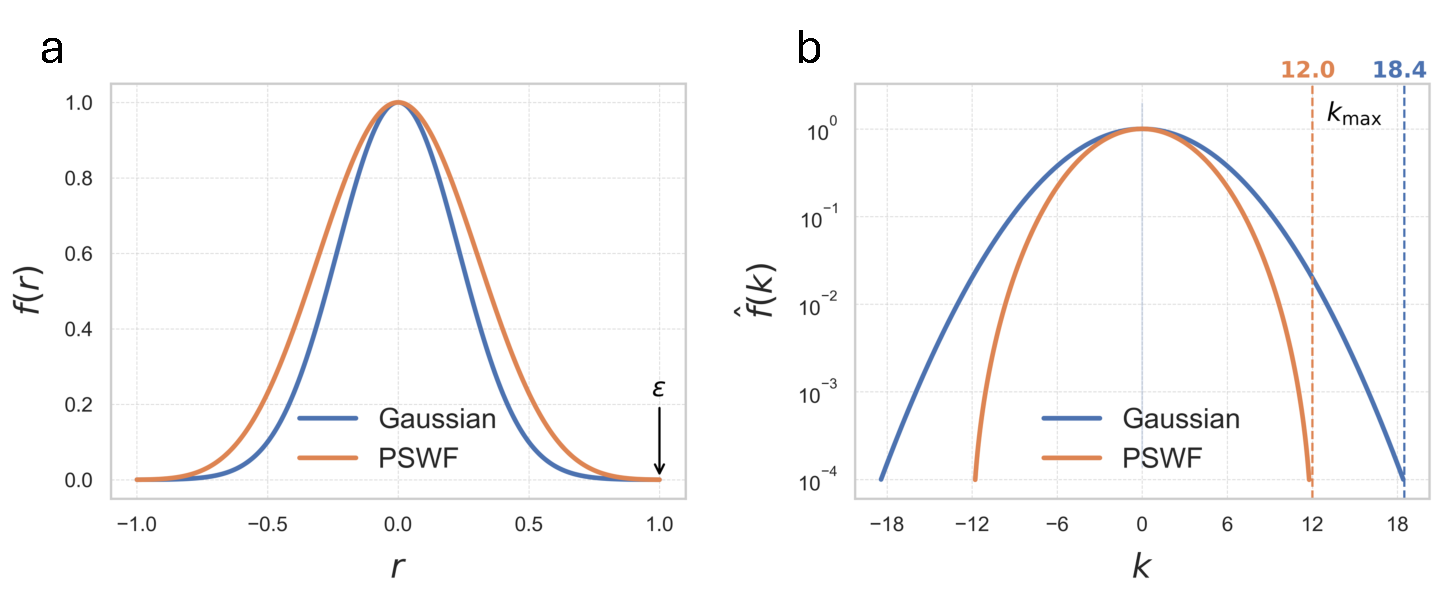
\includegraphics[width=0.78\textwidth]{pswf_gaussian_fourier_transform.pdf}\\[-1mm]
{\scriptsize\gray{The PSWF is the concentration-optimal reference window.}}
\end{center}
\end{column}
\end{columns}
\end{frame}

%================================================================
\begin{frame}{Common compact spreading kernels}
\footnotesize
\begin{center}
\resizebox{0.92\textwidth}{!}{%
\begin{tabular}{@{}lccc@{}}
\toprule
Kernel & defining feature & Fourier correction & implementation note \\
\midrule
Gaussian & analytic in both domains & analytic & historical fast gridding \\
Kaiser--Bessel & compact Bessel window & analytic & established NUFFT/PME option \\
ES & compact semicircle surrogate & numerical / tabulated & legacy GPU option in \texttt{cufinufft} \\
Prolate \(\psi_0^c\) & concentration-optimal window & self-similar finite transform & CPU \texttt{finufft} SI kernel \\
\bottomrule
\end{tabular}
}
\end{center}
\vspace{2mm}
\begin{itemize}
  \item These kernels have different error constants and implementation choices; raw closed-form evaluation cost does not determine performance.
  \item Production SI kernels are evaluated through tables or piecewise polynomials. CPU \texttt{finufft} uses a prolate/PSWF SI kernel.
\end{itemize}
\end{frame}

%================================================================
\begin{frame}{Complexity and parameters}
\small
For \(M\) nonuniform points and \(n^d\) modes in \(d\) dimensions:
\[
  \boxed{\ \cO\big(\sigma^d n^d\log(\sigma n)\big)\ +\ \cO\big(M\,w^d\big)\ }
\]
\begin{itemize}
  \item First term: the FFT on the oversampled grid.
  \item Second term: local spread/interpolate over \(w^d\) nearby grid points per source.
  \item \hl{Precision enters only through \(w\) and \(\sigma\)} --- the asymptotic order is unchanged.
\end{itemize}
\begin{block}{Practical parameter choice}
Use the library's tolerance-to-width rule for its selected kernel, then benchmark the full transform on the target grid, hardware, and point distribution.
\end{block}
\end{frame}

%================================================================
\begin{frame}{Higher dimensions and type 3}
\small
\begin{columns}[T,totalwidth=\textwidth]
\begin{column}{0.52\textwidth}
\textbf{Tensor product.} Widely used multidimensional SI kernels are products,
\[
  \psi(\x)=\prod_{i=1}^d \psi(x_i),
\]
so spreading is a tensor product; the FFT is \(d\)-dimensional. Everything above carries over verbatim, with \(w^d\) local work.
\end{column}
\begin{column}{0.48\textwidth}
\textbf{Type 3 = 1 then 2.}
\begin{itemize}\itemsep2pt
  \item Rescale/shift \(\x_j\) and \(\svec_k\) into boxes.
  \item Type-1 spread of \(c_j\) onto a fine grid sized to the \emph{product} of the two spreads.
  \item Multiply by the (smooth) kernel correction.
  \item Type-2 evaluate at the \(\svec_k\).
\end{itemize}
\end{column}
\end{columns}
\vspace{2mm}
\begin{block}{Reusable computational primitive}
The NUFFT converts exponential sums with scattered nodes into an FFT plus
localized interpolation work; the accuracy is controlled by the oversampling
factor and kernel width.
\end{block}
\end{frame}

%================================================================
\begin{frame}{Software: \texttt{finufft} / \texttt{cufinufft}}
\small
\begin{columns}[T,totalwidth=\textwidth]
\begin{column}{0.58\textwidth}
\begin{itemize}
  \item Types 1,2,3 in 1D/2D/3D; single \& double precision.
  \item Inputs: points \(\x_j\), strengths \(c_j\) (or modes \(f_k\)), a sign,
  and a tolerance \(\epsilon\).
  \item CPU \texttt{finufft} uses a prolate/PSWF SI kernel, evaluated by piecewise polynomial Horner rules; \texttt{cufinufft} keeps the legacy ES GPU kernel.
  \item Multithreaded (CPU) and GPU (\texttt{cufinufft}); interfaces in C/Fortran/MATLAB/Python/Julia.
  \item Tutorial and math notes: \texttt{finufft.readthedocs.io}.
\end{itemize}
\end{column}
\begin{column}{0.42\textwidth}
\footnotesize
\begin{block}{Interface pattern}
Type 1 accepts scattered nodes and strengths, then returns uniform Fourier modes. Type 2 accepts uniform modes and returns values at scattered nodes. The public APIs expose the sign and requested tolerance explicitly.
\end{block}
\end{column}
\end{columns}
\vspace{1mm}
{\scriptsize\gray{References: Dutt \& Rokhlin, \emph{SIAM J.\ Sci.\ Comput.}\ 14 (1993); Greengard \& Lee, \emph{SIAM Review} 46 (2004); Barnett, Magland \& af Klinteberg, \emph{SIAM J.\ Sci.\ Comput.}\ 41 (2019).}}
\end{frame}

%================================================================
\begin{frame}{Where the NUFFT shows up}
\small
\begin{columns}[T,totalwidth=\textwidth]
\begin{column}{0.5\textwidth}
\hl{Imaging / signal processing}
\begin{itemize}\itemsep2pt
  \item MRI \& CT reconstruction (non-Cartesian \(k\)-space).
  \item Radio interferometry (VLA, ALMA), synthetic-aperture radar.
  \item Diffraction, ptychography, cryo-EM.
\end{itemize}
\end{column}
\begin{column}{0.5\textwidth}
\hl{Scientific computing}
\begin{itemize}\itemsep2pt
  \item Fast Ewald / PME (Part II).
  \item Free-space convolution and Fourier quadrature.
  \item Spectral methods on scattered nodes; NUFFT-based quadrature.
\end{itemize}
\end{column}
\end{columns}
\vspace{3mm}
\centerline{\gray{The NUFFT converts between scattered samples and Fourier representations.}}
\end{frame}

%================================================================
\begin{frame}{The fast sinc transform / off-grid interpolation}
\small
The type-2 transform is exactly evaluation of a band-limited function at scattered points --- \hl{trigonometric interpolation off the grid}:
\[
  c_j = \sum_{k} f_k\, e^{\ii k x_j} = P(x_j).
\]
\begin{itemize}
  \item Type 1 followed by type 2 applies a \hl{sinc / DFT interpolation matrix} in \(\cO(n\log n + Mw)\) instead of \(\cO(nM)\).
  \item Basis for NUFFT-accelerated quadrature: to evaluate \(\int f(x)e^{\ii kx}\dd x\) with a nonuniform rule, spread the weighted nodes and FFT.
  \item Exactly this appears next: the Ewald reciprocal sum is a weighted off-grid trigonometric interpolation.
\end{itemize}
\end{frame}

%================================================================
\begin{frame}{NUFFT summary}
\small
\begin{center}
\begin{tikzpicture}[>=Latex,scale=0.9,transform shape,node distance=6mm]
  \node[draw,rounded corners=2pt,fill=black!4,inner sep=5pt] (a){scattered exponential sum};
  \node[draw,rounded corners=2pt,fill=black!4,inner sep=5pt,right=8mm of a] (b){spread with $\psi$};
  \node[draw,rounded corners=2pt,fill=black!4,inner sep=5pt,right=8mm of b] (c){FFT on $\sigma n$ grid};
  \node[draw,rounded corners=2pt,fill=black!4,inner sep=5pt,right=8mm of c] (d){divide by $\widehat\psi$};
  \draw[->,thick,CCMorange](a)--(b);\draw[->,thick,CCMorange](b)--(c);\draw[->,thick,CCMorange](c)--(d);
\end{tikzpicture}
\end{center}
\begin{itemize}
  \item Three transforms (1,2,3); types 1 and 2 are adjoints and share code.
  \item Error \(=\) truncation \(+\) aliasing; both exponentially small, controlled by width \(w\) and oversampling \(\sigma\).
  \item Cost \(\cO(\sigma^d n^d\log n + M w^d)\); precision only changes \(w,\sigma\).
  \item Kernel matters: Gaussian \(\to\) Kaiser--Bessel/ES surrogates \(\to\) prolate (optimal).
\end{itemize}
\vspace{1mm}
\centerline{\hl{Next: the NUFFT accelerates the reciprocal sum in fast Ewald.}}
\end{frame}

%################################################################
\section{Part II: Fast Ewald Summation and ESP}
%################################################################

\begin{frame}{Periodic electrostatics and Ewald summation}
\small
Molecular dynamics, materials, and plasma simulations need the electrostatic energy/forces of \(N\) charges \(q_j\) at positions \(\rr_j\) in a box \(\Omega=[0,L)^3\), \hl{periodically replicated}:
\[
  u(\rr_i)=\sum_{\nnn\in\Z^3}\ \sideset{}{'}\sum_{j=1}^{N}\frac{q_j}{|\rr_i-\rr_j+\nnn L|},
\]
(the prime omits the \(j=i,\ \nnn=\bm0\) self term).
\begin{itemize}
  \item The direct particle--image formulation is both expensive and conditionally convergent.
  \item Ewald summation rewrites it as a short-range real-space contribution and a smooth reciprocal-space contribution.
\end{itemize}
\begin{block}{This block}
Classical Ewald \(\Rightarrow\) mesh Ewald (PME/SPME) as gridded Fourier
summation \(\Rightarrow\) ESP: replace Gaussians and B-splines by prolates for
smaller reciprocal grids.
\end{block}
{\scriptsize\gray{P.\ Ewald, \emph{Annalen der Physik} 369 (1921); T.\ Darden, D.\ York \& L.\ Pedersen, \emph{Journal of Chemical Physics} 98 (1993).}}
\end{frame}

%================================================================
\begin{frame}{The lattice sum and its convergence}
\small
The energy is a sum over all periodic images,
\[
  E=\frac12\sum_{\nnn\in\Z^3}\ \sideset{}{'}\sum_{i,j}\frac{q_iq_j}{|\rr_{ij}+\nnn L|}.
\]
\begin{itemize}
  \item Terms decay like \(1/r\); the sum is \hl{only conditionally convergent} --- value depends on summation order and the medium at infinity.
  \item Direct truncation converges painfully slowly and is inaccurate.
  \item Ewald's resolution: rewrite as \emph{two} absolutely (and rapidly) convergent sums, one per space.
\end{itemize}
\end{frame}

%================================================================
\begin{frame}{Ewald splitting: screen, then correct}
\footnotesize
Around each point charge, add and subtract a smooth \hl{screening cloud} (a Gaussian of width \(\sim 1/\alpha\)):
\begin{itemize}
  \item Point charge \(+\) opposite-sign smooth cloud \(=\) a \hl{short-ranged} object \(\Rightarrow\) sum in \hl{real space}.
  \item The compensating smooth clouds form a \hl{smooth periodic density} \(\Rightarrow\) sum in \hl{reciprocal space} (few Fourier modes).
\end{itemize}
Algebraically this is the kernel split
\[
  \frac1r=\underbrace{\frac{\erf(\alpha r)}{r}}_{\text{smooth, long range}}+\underbrace{\frac{\erfc(\alpha r)}{r}}_{\text{singular, short range}} .
\]
\begin{center}
\begin{tikzpicture}[
  x=0.92cm,y=0.82cm,
  axis/.style={->,black!70,line width=0.45pt},
  tick/.style={black!70,line width=0.35pt},
  guide/.style={black!12,line width=0.25pt}
]
  \def\xmax{4.15}
  \def\ymax{2.55}
  \begin{scope}
    \node[anchor=south] at (2.05,2.70) {\scriptsize original kernel};
    \foreach \xv in {1,2,3,4} \draw[guide] (\xv,0)--(\xv,2.45);
    \foreach \yv in {1,2} \draw[guide] (0,\yv)--(4.05,\yv);
    \draw[axis] (0,0)--(\xmax,0) node[below right]{\scriptsize $r$};
    \draw[axis] (0,0)--(0,\ymax) node[above left]{\scriptsize $K(r)$};
    \foreach \xv in {1,2,3,4} \draw[tick] (\xv,0)--(\xv,-0.06) node[below]{\scriptsize \(\xv\)};
    \foreach \yv in {1,2} \draw[tick] (0,\yv)--(-0.06,\yv) node[left]{\scriptsize \(\yv\)};
    \draw[thick,SFdark] plot[smooth,domain=0.36:4.05,samples=80]({\x},{0.9/\x});
    \node[SFdark,fill=white,inner sep=1pt] at (1.05,1.92){\scriptsize $1/r$};
  \end{scope}
  \begin{scope}[shift={(5.35,0)}]
    \node[anchor=south] at (2.05,2.70) {\scriptsize split pieces};
    \foreach \xv in {1,2,3,4} \draw[guide] (\xv,0)--(\xv,2.45);
    \foreach \yv in {1,2} \draw[guide] (0,\yv)--(4.05,\yv);
    \draw[axis] (0,0)--(\xmax,0) node[below right]{\scriptsize $r$};
    \draw[axis] (0,0)--(0,\ymax) node[above left]{\scriptsize $K(r)$};
    \foreach \xv in {1,2,3,4} \draw[tick] (\xv,0)--(\xv,-0.06) node[below]{\scriptsize \(\xv\)};
    \foreach \yv in {1,2} \draw[tick] (0,\yv)--(-0.06,\yv) node[left]{\scriptsize \(\yv\)};
    \draw[thick,CCMorange] plot[smooth,domain=0.05:4.05,samples=100]
      ({\x},{0.9*sqrt(1-exp(-(\x)^2*(4/pi+0.147*(\x)^2)/(1+0.147*(\x)^2)))/\x});
    \node[CCMorange,fill=white,inner sep=1pt] at (2.18,0.90){\scriptsize $\erf(\alpha r)/r$};
    \draw[thick,SFdark] plot[smooth,domain=0.36:4.05,samples=100]
      ({\x},{0.9*(1-sqrt(1-exp(-(\x)^2*(4/pi+0.147*(\x)^2)/(1+0.147*(\x)^2))))/\x});
    \node[SFdark,fill=white,inner sep=1pt] at (1.02,1.64){\scriptsize $\erfc(\alpha r)/r$};
  \end{scope}
\end{tikzpicture}
\end{center}
\end{frame}

%================================================================
\begin{frame}{The real-space (short-range) sum}
\small
The complementary-error part is negligible beyond a cutoff \(r_c\) (\(\erfc(\alpha r_c)\le\epsilon\)):
\[
  E_{\rm real}=\frac12\sum_{\nnn}\ \sideset{}{'}\sum_{i,j}
     q_i q_j\,\frac{\erfc(\alpha|\rr_{ij}+\nnn L|)}{|\rr_{ij}+\nnn L|}.
\]
\begin{itemize}
  \item With a neighbor list, each charge interacts with \(\cO(1)\) others \(\Rightarrow\) \hl{\(\cO(N)\)} cost.
  \item Larger \(\alpha\) (thinner clouds) \(\Rightarrow\) shorter real-space cutoff, but \emph{more} Fourier modes needed. This is the fundamental Ewald trade-off.
  \item This is the single-level analog of the residual/local kernels that
  appear at many levels in DMK.
\end{itemize}
\end{frame}

%================================================================
\begin{frame}{The reciprocal-space (long-range) sum}
\small
The smooth part is a periodic function; expand it in a Fourier series over \(\kk=\tfrac{2\pi}{L}\mm\), \(\mm\in\Z^3\):
\[
  E_{\rm recip}=\frac{1}{2L^3}\sum_{\kk\neq \bm0}\frac{4\pi}{k^2}\,e^{-k^2/4\alpha^2}\,\big|S(\kk)\big|^2,
  \qquad
  S(\kk)=\sum_{j=1}^N q_j\, e^{\ii\kk\cdot\rr_j}.
\]
\begin{itemize}
  \item \(S(\kk)\) is the \hl{structure factor}; the Gaussian factor \(e^{-k^2/4\alpha^2}\) truncates the sum to \(|\kk|\lesssim 2\alpha\sqrt{\log(1/\epsilon)}\).
  \item \(S(\kk)\) is a \hl{type-1 sum} (charges at nonuniform \(\rr_j\) \(\to\) modes \(\kk\)); evaluating \(\sum_{\kk}(\cdots)e^{-\ii\kk\cdot\rr_i}\) at the targets is a \hl{type-2 sum}.
  \item The \(k=0\) term is dropped: it requires overall \hl{charge neutrality}, \(\sum_j q_j=0\).
\end{itemize}
\end{frame}

%================================================================
\begin{frame}{Deriving the reciprocal sum}
\small
The smooth part is convolution of the charge density with a Gaussian-screened kernel. On a periodic box, expand in a Fourier series (Poisson summation): with density \(\rho(\rr)=\sum_j q_j\delta(\rr-\rr_j)\),
\[
  \widehat\rho(\kk)=\sum_j q_j e^{\ii\kk\cdot\rr_j}=S(\kk),\qquad
  \widehat{\mathcal S}(\kk)=\frac{4\pi}{k^2}e^{-k^2/4\alpha^2}.
\]
Parseval then gives the energy as a sum over reciprocal lattice vectors \(\kk=\tfrac{2\pi}{L}\mm\):
\[
  E_{\rm recip}=\frac{1}{2L^3}\sum_{\kk\neq\bm0}\widehat{\mathcal S}(\kk)\,|S(\kk)|^2 .
\]
\begin{itemize}
  \item The \hl{structure factor} \(S(\kk)\) bundles all \(N\) charges into each mode --- a type-1 sum.
  \item The Gaussian factor truncates the series to \(\cO((\alpha L)^3)\) modes.
\end{itemize}
\end{frame}

%================================================================
\begin{frame}{The self-energy correction}
\small
The reciprocal sum includes each charge interacting with its \emph{own} smooth cloud. Subtract it:
\[
  E_{\rm self}=-\frac{\alpha}{\sqrt\pi}\sum_{j=1}^{N}q_j^2 .
\]
So the total electrostatic energy is
\[
  E=\underbrace{E_{\rm real}}_{\erfc,\ \text{real space}}+\underbrace{E_{\rm recip}}_{\text{Fourier}}+\underbrace{E_{\rm self}}_{\text{constant}}\ (+\ \text{net-charge / surface terms}).
\]
\begin{itemize}
  \item The self term follows from \(\displaystyle \lim_{r\to0}\frac{\erf(\alpha r)}{r}=\frac{2\alpha}{\sqrt\pi}\): the smooth kernel is finite at the origin.
  \item Non-neutral cells need a uniform neutralizing background (a \(k=0\) correction).
  \item Everything is analytic --- the only approximation is truncating the two rapidly convergent sums.
\end{itemize}
\end{frame}

%================================================================
\begin{frame}{Classical Ewald: cost and the optimal split}
\small
Balancing the two sums fixes \(\alpha\):
\begin{itemize}
  \item Real space: cost \(\propto N\cdot(\alpha^{-1})^3\) (charges within the cutoff).
  \item Reciprocal space: number of modes \(\propto (\alpha L)^3\); direct evaluation of \(S(\kk)\) at all modes is \(\cO(N\cdot N_F)\).
  \item Choosing \(\alpha\sim N^{1/6}/L\) balances them \(\Rightarrow\) classical Ewald is \hl{\(\cO(N^{3/2})\)}.
\end{itemize}
\begin{block}{The opportunity}
\(S(\kk)\) and its adjoint are type-1 / type-2 nonuniform Fourier sums.
Replacing the direct \(\cO(N\,N_F)\) evaluation by gridding + FFT, or by a
modern NUFFT, gives the particle-mesh Ewald idea.
\end{block}
\end{frame}

%================================================================
\begin{frame}{A general kernel-splitting view}
\small
Write the Coulomb kernel with an even, normalized \hl{screening function} \(\chi\), \(\int_0^\infty\chi(t)\dd t=1\):
\[
  \begin{aligned}
  \frac{1}{4\pi r}&=\mathcal S(r)+\mathcal L(r),\\
  \mathcal S(r)&=\frac{\int_0^{r/r_c}\chi(t)\dd t}{4\pi r}\quad (\text{smooth, long range}),\\
  \mathcal L(r)&=\frac{1-\int_0^{r/r_c}\chi(t)\dd t}{4\pi r}\quad (\text{local}).
  \end{aligned}
\]
\begin{itemize}
  \item \(\chi(t)=\tfrac{2\eta}{\sqrt\pi}e^{-\eta^2t^2}\), with \(\eta=\alpha r_c\), recovers the \(\erf/\erfc\) split.
  \item \(\mathcal L\) is evaluated directly after truncation at the requested tolerance.
  \item \(\mathcal S\) is done in Fourier space --- and that is where NUFFT/FFT enters.
\end{itemize}
\end{frame}

%================================================================
\begin{frame}{From Ewald to Particle-Mesh Ewald (PME/SPME/PPPM)}
\small
Write the smooth Coulomb kernel as a general split \(\tfrac{1}{4\pi r}=\mathcal S(r)+\mathcal L(r)\) with a screening function \(\chi_\alpha\); the long-range potential is
\[
  u_i^{s}\approx\sum_{\substack{\kk\in\mathcal I\\ \kk\neq\bm0}}
  e^{-\ii\kk\cdot\rr_i}\ \frac{\widehat{\mathcal S}(\kk)}{L^3}
  \sum_{j=1}^{N}e^{\ii\kk\cdot\rr_j}q_j .
\]
\begin{itemize}
  \item \hl{Inner sum:} nonuniform sources \(\rr_j\) \(\to\) uniform modes \(\kk\) \(=\) \hl{type-1 NUFFT}.
  \item \hl{Outer sum:} uniform modes \(\kk\) \(\to\) nonuniform targets \(\rr_i\) \(=\) \hl{type-2 NUFFT}.
  \item Historically PME/PPPM used B-spline spreading + FFT; modern NUFFT language is a clean way to view the same reciprocal-space acceleration.
\end{itemize}
\end{frame}

%================================================================
\begin{frame}{The five-step spreading--interpolation procedure}
\small
With a spreading/interpolation (SI) kernel \(\phi\), grid spacing \(h=L/n_f\):
\[
\begin{array}{rll}
\text{(1) \hl{Spread}}: & b_{\bm\ell}=\sum_{j=1}^N \tilde\phi(\rr_j-h\bm\ell)\,q_j, & \bm\ell\in\mathcal I\\[3pt]
\text{(2) \hl{FFT}}: & \hat b_{\kk}=\sum_{\bm\ell} e^{2\pi\ii\,\kk\cdot\bm\ell/n_f} b_{\bm\ell}, & \kk\in\mathcal I\\[3pt]
\text{(3) \hl{Scale}}: & \hat c_{\kk}=p_{\kk}\,\hat b_{\kk}, & \kk\in\mathcal I\\[3pt]
\text{(4) \hl{IFFT}}: & c_{\bm\ell'}=\sum_{\kk} e^{-2\pi\ii\,\kk\cdot\bm\ell'/n_f}\hat c_{\kk}, & \bm\ell'\in\mathcal I\\[3pt]
\text{(5) \hl{Interpolate}}: & \tilde u_i^s=\sum_{\bm\ell'}\tilde\phi(\rr_i-h\bm\ell')\,c_{\bm\ell'}, & i=1,\dots,N
\end{array}
\]
\begin{itemize}
  \item Steps (1)--(2): type-1 NUFFT. Steps (4)--(5): type-2 NUFFT. Step (3): a diagonal Fourier multiplier.
  \item Cost \(\cO(N P^3)+\cO(N_f\log N_f)\), \(N_f=\cO(N)\), where \(P\) is the SI width.
\end{itemize}
\end{frame}

%================================================================
\begin{frame}{The diagonal multiplier and two accuracy parameters}
\small
The scaling factor in step (3) carries the physics and undoes the spreading:
\[
  p_{\kk}=\frac{\widehat{\mathcal S}(2\pi\kk/L)}{L^3\,|\widehat\phi(2\pi\kk/L)|^2}
        =\frac{\widehat\chi\!\big(2\pi r_c|\kk|/L\big)}{2\pi L\,|\widehat\phi(2\pi\kk/L)|^2\,|\kk|^2}.
\]
\begin{itemize}
  \item Numerator: the smooth Ewald kernel in Fourier space (the Gaussian screen).
  \item Denominator \(|\widehat\phi|^2\): deconvolves the \emph{two} SI operations (spread and interpolate).
  \item \hl{Two accuracy parameters}: the SI width \(P\), and the grid size \(n_f\)
  (oversampling), as in the NUFFT analysis.
\end{itemize}
\begin{block}{The cost driver}
\(n_f\) sets the FFT size and the communication cost on parallel machines. \emph{Smaller grid at equal accuracy \(=\) faster MD.} This is what ESP attacks.
\end{block}
\end{frame}

%================================================================
\begin{frame}{The mesh-Ewald family (PPPM / PME / SPME)}
\small
All ``mesh Ewald'' methods accelerate the \emph{same} reciprocal sum by gridding:
\begin{itemize}\itemsep2pt
  \item \hl{PPPM} \gray{(Hockney--Eastwood 1988)}: particle--particle / particle--mesh split; the ancestor.
  \item \hl{PME} \gray{(Darden--York--Pedersen 1993)}: Lagrange interpolation of \(e^{\ii\kk\cdot\rr}\) onto the grid.
  \item \hl{SPME} \gray{(Essmann et al.\ 1995)}: smooth B-spline interpolation \(\Rightarrow\) analytic forces (differentiate the spline).
\end{itemize}
\vspace{1mm}
\begin{block}{Forces as the accuracy target}
MD needs \(\bm F_i=-\nabla_{\rr_i}E\). With a smooth SI kernel the gradient passes onto the spreading step; the FFT work is shared between energy and forces. Accuracy in the \emph{force} is what actually matters.
\end{block}
\end{frame}

%================================================================
\begin{frame}{Ewald parameter selection}
\small
Three coupled parameters trade off, for target accuracy \(\epsilon\):
\begin{itemize}\itemsep2pt
  \item \hl{splitting \(\alpha\)} (or \(\sigma=1/\alpha\)): sets the real-space cutoff \(r_c\) via \(\erfc(\alpha r_c)\le\epsilon\).
  \item \hl{grid size \(n_f\)}: must resolve the screened density; \(n_f\propto \alpha L\).
  \item \hl{SI width \(P\)}: sets the aliasing floor at fixed \(n_f\).
\end{itemize}
\[
  \text{real-space} \sim N\,(\alpha^{-1})^3,\qquad \text{reciprocal} \sim n_f^3\log n_f + N P^3 .
\]
\begin{block}{Reciprocal-grid cost driver}
On a parallel machine the 3D FFT needs global all-to-all communication. \(n_f\) --- not \(P\) or \(r_c\) --- often dominates the wall-clock. Shrinking \(n_f\) is therefore a high-value optimization.
\end{block}
\end{frame}

%================================================================
\begin{frame}{Classical choices and their limitation}
\small
\begin{columns}[T,totalwidth=\textwidth]
\begin{column}{0.5\textwidth}
\textbf{Standard PME / SPME}
\[
  \chi(r)=\tfrac{2}{\sqrt\pi}e^{-\alpha r^2},\quad
  \widehat\phi(\bm\xi)=\prod_{i}\Big(\tfrac{\sin(\xi_i h/2)}{\xi_i h/2}\Big)^{P}.
\]
\begin{itemize}\itemsep2pt
  \item \hl{Gaussian} screen (Ewald 1921).
  \item \hl{B-splines} as the SI kernel (PPPM/PME/SPME).
  \item Parameters are chosen from the target force tolerance and cutoff;
  typically \(n_f\) grows like \((L/r_c)\log(1/\epsilon)\).
\end{itemize}
\end{column}
\begin{column}{0.5\textwidth}
\textbf{Why it is not optimal}
\begin{itemize}\itemsep3pt
  \item B-splines have slowly decaying transforms \(\Rightarrow\) large aliasing unless the grid \(n_f\) is big.
  \item The Gaussian is not the best-concentrated band-limited window.
  \item Result: \emph{larger FFTs than necessary}, and more MPI communication.
\end{itemize}
\end{column}
\end{columns}
\vspace{2mm}
\centerline{\hl{Both choices can be replaced by one object: the prolate spheroidal wave function.}}
\end{frame}

%================================================================
\begin{frame}{ESP: Ewald Summation with Prolates}
\small
\gray{J.\ Liang, L.\ Lu, A.\ Barnett, L.\ Greengard \& S.\ Jiang, \emph{Nature Communications} 17 (2026), doi:10.1038/s41467-026-73232-8.}
\begin{columns}[T,totalwidth=\textwidth]
\begin{column}{0.5\textwidth}
Replace \emph{both} classical choices by the zeroth prolate \(\psi_0^c\):
\[
  \begin{aligned}
  \chi(x)&=\frac{\psi_0^c(x)}{C_0}, & C_0&=\int_{-1}^{1}\psi_0^c(t)\dd t,\\
  \phi(\x)&=\prod_{i=1}^3 \psi_0^{c_1}\!\Big(\tfrac{2x_i}{Ph}\Big).
  \end{aligned}
\]
\end{column}
\begin{column}{0.5\textwidth}
\begin{itemize}\itemsep2pt
  \item Prolate for the \hl{kernel split} (instead of Gaussian).
  \item Prolate for the \hl{SI kernel} (instead of B-splines).
  \item Choose \(c\) so \(\psi_0^c(1)=\epsilon\Rightarrow c\approx\log(1/\epsilon)\).
\end{itemize}
\end{column}
\end{columns}
\vspace{2mm}
The prolate's Fourier support is essentially \([-c,c]\), giving the grid size
\[
  n_f=\Big\lceil \frac{cL}{\pi r_c}\Big\rceil,
\]
\hl{noticeably smaller} than the B-spline/Gaussian value at the same accuracy.
\end{frame}

%================================================================
\begin{frame}{Prolate spheroidal wave functions}
\footnotesize
\setlength{\abovedisplayskip}{3pt}
\setlength{\belowdisplayskip}{3pt}
For bandwidth \(c>0\), the PSWFs \(\psi_0^c,\psi_1^c,\dots\) are the eigenfunctions of the finite Fourier transform on \([-1,1]\),
\[
  F_c[\phi](x)=\int_{-1}^1\phi(t)\,e^{\ii cxt}\dd t=\lambda_n\,\psi_n^c(x).
\]
\vspace{-1mm}
\begin{itemize}\itemsep2pt
  \item Real, orthonormal, complete in \(L^2[-1,1]\); \(\psi_0^c\) is even and sign-definite.
  \item \(|\lambda_n|\) stay \(\cO(1)\) until \(n\approx 2c/\pi\), then decay rapidly: the time--bandwidth degrees of freedom.
  \item Precise concentration statement: among unit \(L^2[-1,1]\) functions, \(\psi_0^c\) maximizes Fourier energy in the band \([-c,c]\).
\end{itemize}
\vspace{-1mm}
\begin{center}
\begin{tabular}{@{}c@{\hspace{7mm}}c@{}}
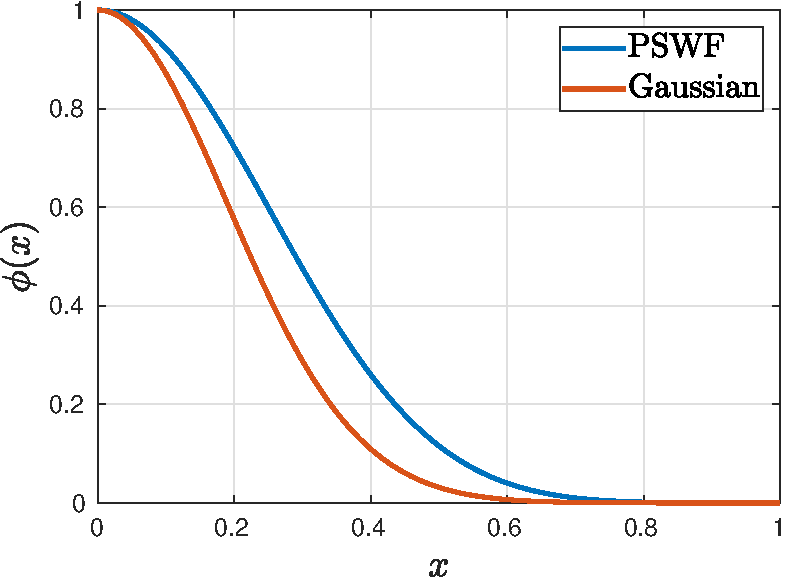
\includegraphics[height=29mm]{pswfgaussian.pdf} &
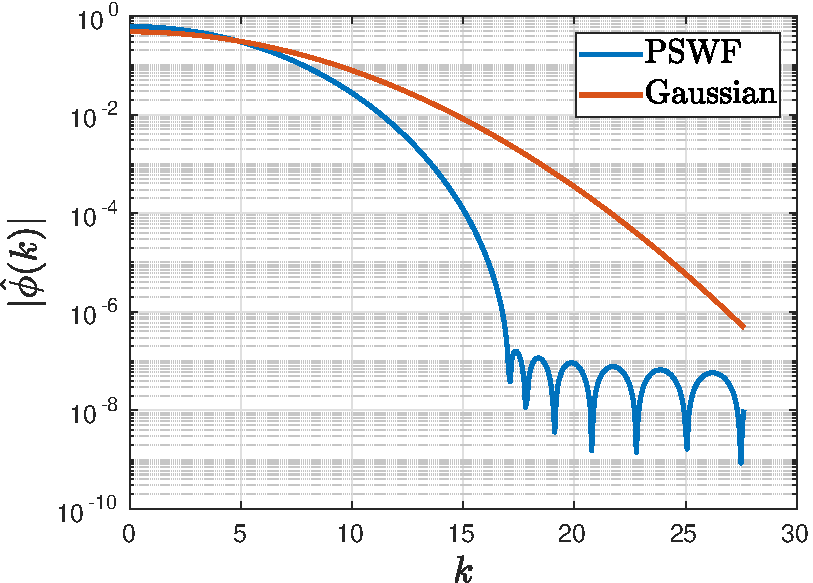
\includegraphics[height=29mm]{pswfgaussianfouriertransform.pdf}\\[-1mm]
{\scriptsize\gray{physical space}} &
{\scriptsize\gray{Fourier space}}
\end{tabular}
\end{center}
\end{frame}

%================================================================
\begin{frame}{Prolates as optimal concentration windows}
\small
The zeroth prolate \(\psi_0^c\) is the principal eigenfunction of the finite Fourier transform
\[
  \int_{-1}^1 \psi_0^c(t)\,e^{\ii c x t}\dd t=\lambda_0\,\psi_0^c(x),
\]
and it solves the precise variational problem
\[
  \psi_0^c=\underset{\substack{f\in L^2[-1,1]\\\|f\|_2=1}}{\operatorname{argmax}}\
  \int_{-1}^{1}\left|\int_{-1}^{1} f(t)e^{\ii cxt}\dd t\right|^2\dd x .
\]
\begin{itemize}
  \item This is exactly the concentration property needed by a spreading/interpolation window: retain as much spectral energy as possible inside the resolved band.
  \item The finite Fourier transform maps \(\psi_0^c\) back to a scaled copy of itself on \([-1,1]\).
  \item In ESP and CPU \texttt{finufft}, the function is evaluated through piecewise-polynomial approximations.
\end{itemize}
\end{frame}

%================================================================
\begin{frame}{Grid-size reduction from ESP}
\small
Optimal parameters from the ESP paper: Gaussian shape parameter \(\alpha_{\rm G}\), prolate bandwidth \(c_{\rm pswf}\), ESP spreading width \(P_{\rm esp}\), and the \hl{grid ratio} \(R_{\rm default}\) at equal accuracy:
\begin{center}
\scriptsize
\begin{tabular}{lccccc}
\toprule
\(\epsilon\) & \(10^{-3}\) & \(5\times10^{-4}\) & \(10^{-4}\) & \(5\times10^{-5}\) & \(10^{-5}\)\\
\midrule
\(\alpha_{\rm G}\) & 6.91 & 7.60 & 9.21 & 9.90 & 11.51\\
\(c_{\rm pswf}\) & 9.54 & 10.29 & 12.02 & 12.76 & 14.47\\
\(P_{\rm esp}\) & 5 & 5 & 6 & 7 & 8\\
\midrule
\(R_{\rm default}\) & 5.78 & \textbf{7.71} & \textbf{14.32} & 22.42 & 54.57\\
\bottomrule
\end{tabular}
\end{center}
\begin{itemize}
  \item \(R_{\rm default}\) is the ratio of the total Fourier-grid size for default PME (with its grid increased until it meets the stated tolerance) to that for ESP.
  \item Smaller grid \(\Rightarrow\) smaller FFT \emph{and} much less MPI communication, often the dominant cost at scale.
\end{itemize}
{\scriptsize\gray{J.\ Liang, L.\ Lu, A.\ Barnett, L.\ Greengard \& S.\ Jiang, \emph{Nature Communications} 17 (2026), doi:10.1038/s41467-026-73232-8, Table 1.}}
\end{frame}

%================================================================
\begin{frame}{ESP in real MD codes}
\small
\begin{itemize}
  \item ESP was implemented and benchmarked in \textsc{Lammps} and \textsc{Gromacs}.
  \item The reported comparisons use equal force tolerances and measure full MD step time as well as the reciprocal-space work.
  \item Fewer Fourier modes reduce both FFT work and global communication; the resulting total speedup depends on system, tolerance, and core count.
\end{itemize}
\vspace{2mm}
\begin{block}{What to look for in the timing plots}
Compare ESP against both the default mesh-Ewald parameters and the best tuned
PME/PPPM baseline.  The relevant metric is total wall time per MD step, not only
the reciprocal-space kernel time.
\end{block}
{\scriptsize\gray{J.\ Liang, L.\ Lu, A.\ Barnett, L.\ Greengard \& S.\ Jiang, \emph{Nature Communications} 17 (2026), doi:10.1038/s41467-026-73232-8.}}
\end{frame}

%================================================================
\begin{frame}{ESP runtime scaling in MD codes}
\footnotesize
\begin{columns}[T,totalwidth=\textwidth]
\begin{column}{0.63\textwidth}
\centering
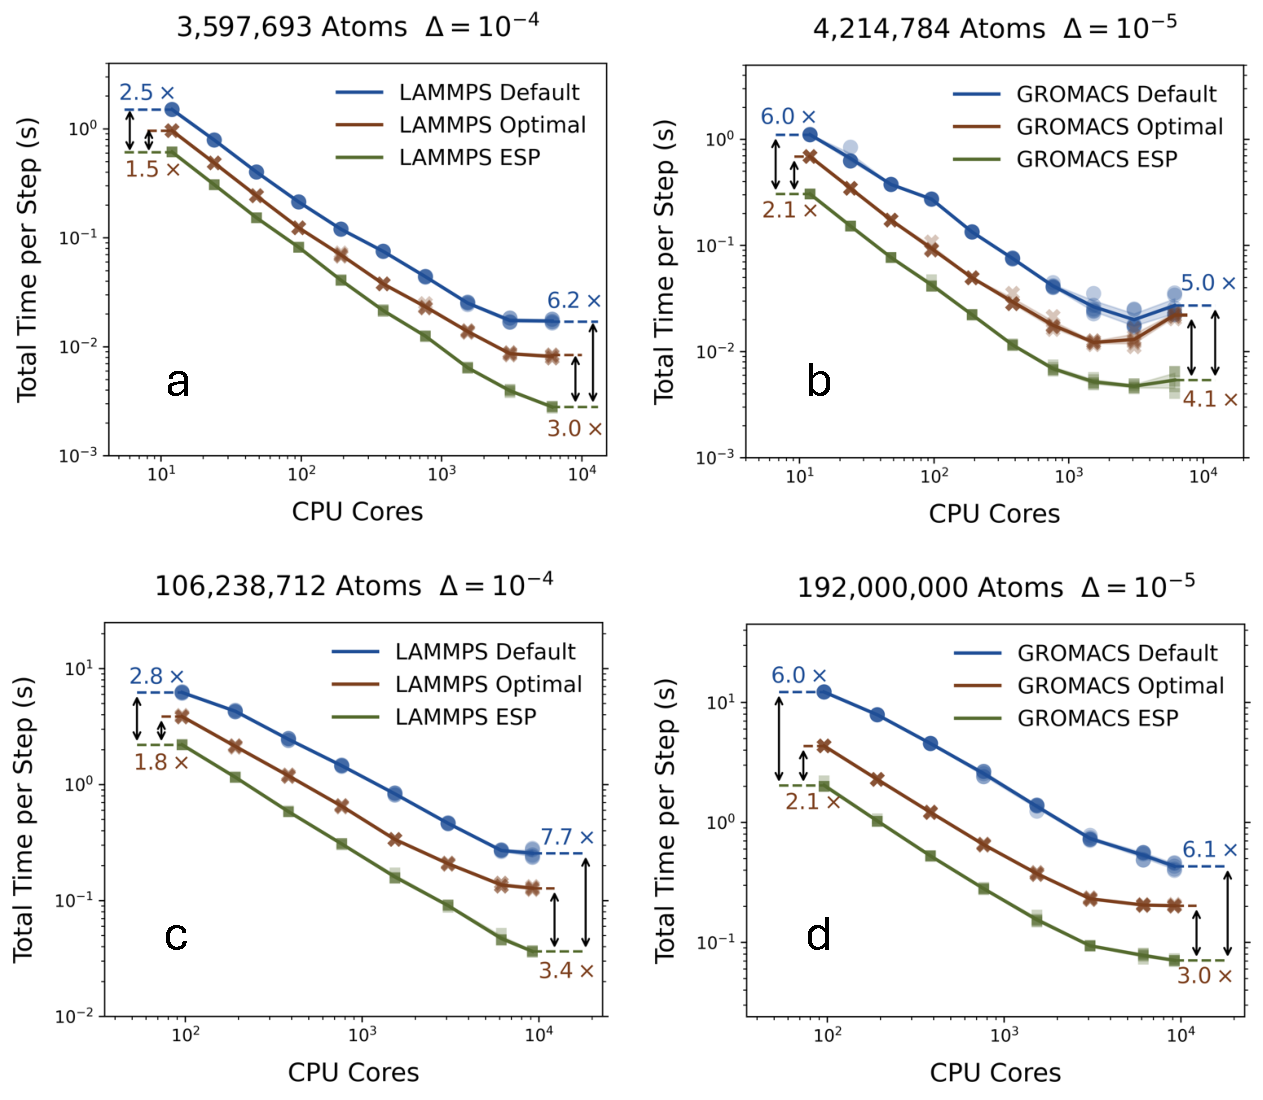
\includegraphics[height=66mm]{Time.pdf}
\end{column}
\begin{column}{0.35\textwidth}
\scriptsize
\textbf{Caption.} Bulk-water strong-scaling tests in \textsc{Lammps} and
\textsc{Gromacs}.
\begin{itemize}\itemsep2pt
  \item Vertical axis: total time per MD step.
  \item Horizontal axis: CPU cores.
  \item Blue: default PME/PPPM; brown: tuned PME/PPPM; green: ESP.
  \item Arrows report total runtime speedups, averaged over 2000 steps.
  \item ``Default'' uses standard \(P=5\).
\end{itemize}
\end{column}
\end{columns}
{\scriptsize\gray{J.\ Liang, L.\ Lu, A.\ Barnett, L.\ Greengard \& S.\ Jiang, \emph{Nature Communications} 17 (2026), doi:10.1038/s41467-026-73232-8.}}
\end{frame}

%================================================================
\begin{frame}{Fast Ewald and ESP summary}
\small
\begin{itemize}
  \item Periodic Coulomb sums are conditionally convergent; \hl{Ewald splits} \(1/r\) into a short-range \(\erfc\) part (real space) and a smooth \(\erf\) part (Fourier space) plus a self term.
  \item Classical Ewald is \(\cO(N^{3/2})\); gridding the reciprocal sum and using FFT/NUFFT gives \hl{PME-type \(\cO(N\log N)\)} methods.
  \item ESP uses the prolate concentration window for both the kernel split and the SI kernel; the paper reports a substantial reduction in Fourier-grid size at matched tolerance.
\end{itemize}
\vspace{2mm}
\begin{block}{Limitation of a single splitting scale}
A single global split and mesh are most efficient for approximately uniform particle densities. A multilevel split provides a different organization for strongly nonuniform distributions, which motivates DMK.
\end{block}
\end{frame}

%================================================================
\begin{frame}{Break}
\centering
\vspace{16mm}
{\Large 10 minute break}

\vspace{8mm}
After the break: the Dual-space Multilevel Kernel-splitting (DMK) framework.

\vspace{4mm}
{\small DMK replaces long interaction lists by local interactions on a hierarchy
of kernel-splitting levels.}
\end{frame}

%################################################################
\section{Part III: The DMK Framework}
%################################################################

\begin{frame}{Dual-space multilevel kernel splitting}
\small
\gray{S.\ Jiang \& L.\ Greengard, \emph{A dual-space multilevel kernel-splitting framework for discrete and continuous convolution}, \emph{Communications on Pure and Applied Mathematics} 78 (2025) 1086--1143.}
\vspace{2mm}

For a broad class of kernels \(K\) and \emph{arbitrary} (possibly highly
nonuniform) points, the target is
\[
  u_i=\sum_{j=1}^N K(\x_i-\y_j)\,\rho_j\ \ (\text{discrete}),\qquad
  u(\x)=\int_B K(\x-\y)\rho(\y)\dd\y\ \ (\text{continuous}),
\]
in \hl{\(\cO(N)\)} work, fully adaptively.
\begin{itemize}
  \item Kernels: Laplace \(1/r\), Yukawa \(e^{-\lambda r}/r\), power functions \(1/r^\alpha\), \(\sqrt{-\Delta}\), Mat\'ern / RBFs, log --- many nonoscillatory kernels.
  \item DMK combines \hl{tree adaptivity} from the FMM viewpoint with
  \hl{Fourier diagonalization} from the Ewald viewpoint.
\end{itemize}
\end{frame}

%================================================================
\begin{frame}{The two classical families of fast algorithms}
\small
\begin{columns}[T,totalwidth=\textwidth]
\begin{column}{0.5\textwidth}
\textbf{Tree-based (FMM \& variants)}
\begin{itemize}\itemsep2pt
  \item Fully \hl{adaptive}, \(\cO(N)\).
  \item Separates near / far field; well-separated interactions are low rank.
  \item Compression uses PDE-specific expansions.
  \item Complex interaction lists (up to \(6^d-3^d\) boxes).
\end{itemize}
\end{column}
\begin{column}{0.5\textwidth}
\textbf{FFT-based (fast Ewald)}
\begin{itemize}\itemsep2pt
  \item \(\cO(N\log N)\), tiny constant.
  \item Diagonalizes convolution in Fourier space.
  \item \hl{Not adaptive}: one scale \(\sigma\) assumes uniformity.
  \item Relies on the FFT.
\end{itemize}
\end{column}
\end{columns}
\vspace{3mm}
\begin{block}{DMK's aim}
Keep the \hl{adaptivity of the FMM} \emph{and} the \hl{Fourier diagonalization
of Ewald}, while reducing interaction lists to nearest-neighbor boxes on each
level and avoiding FFT dependence in the asymptotic complexity.
\end{block}
\end{frame}

%================================================================
\begin{frame}{Reminder: the FMM key observation}
\small
\begin{columns}[T,totalwidth=\textwidth]
\begin{column}{0.55\textwidth}
Sort points into a box tree. When target box \(B_T\) and source box \(B_S\) are \hl{well separated},
\[
  K(\x,\y)\approx\sum_{k=1}^{p}f_k(\x)\,g_k(\y),
\]
a low-rank (separable) approximation with \(p=\cO(\log^s\tfrac1\epsilon)\), \emph{independent of box size}.
\begin{itemize}
  \item Far field compresses; near field is direct.
  \item \(\cO(N)\) via an upward pass (multipole) and downward pass (local), with M2M, M2L, L2L translations.
\end{itemize}
\end{column}
\begin{column}{0.42\textwidth}
\centering
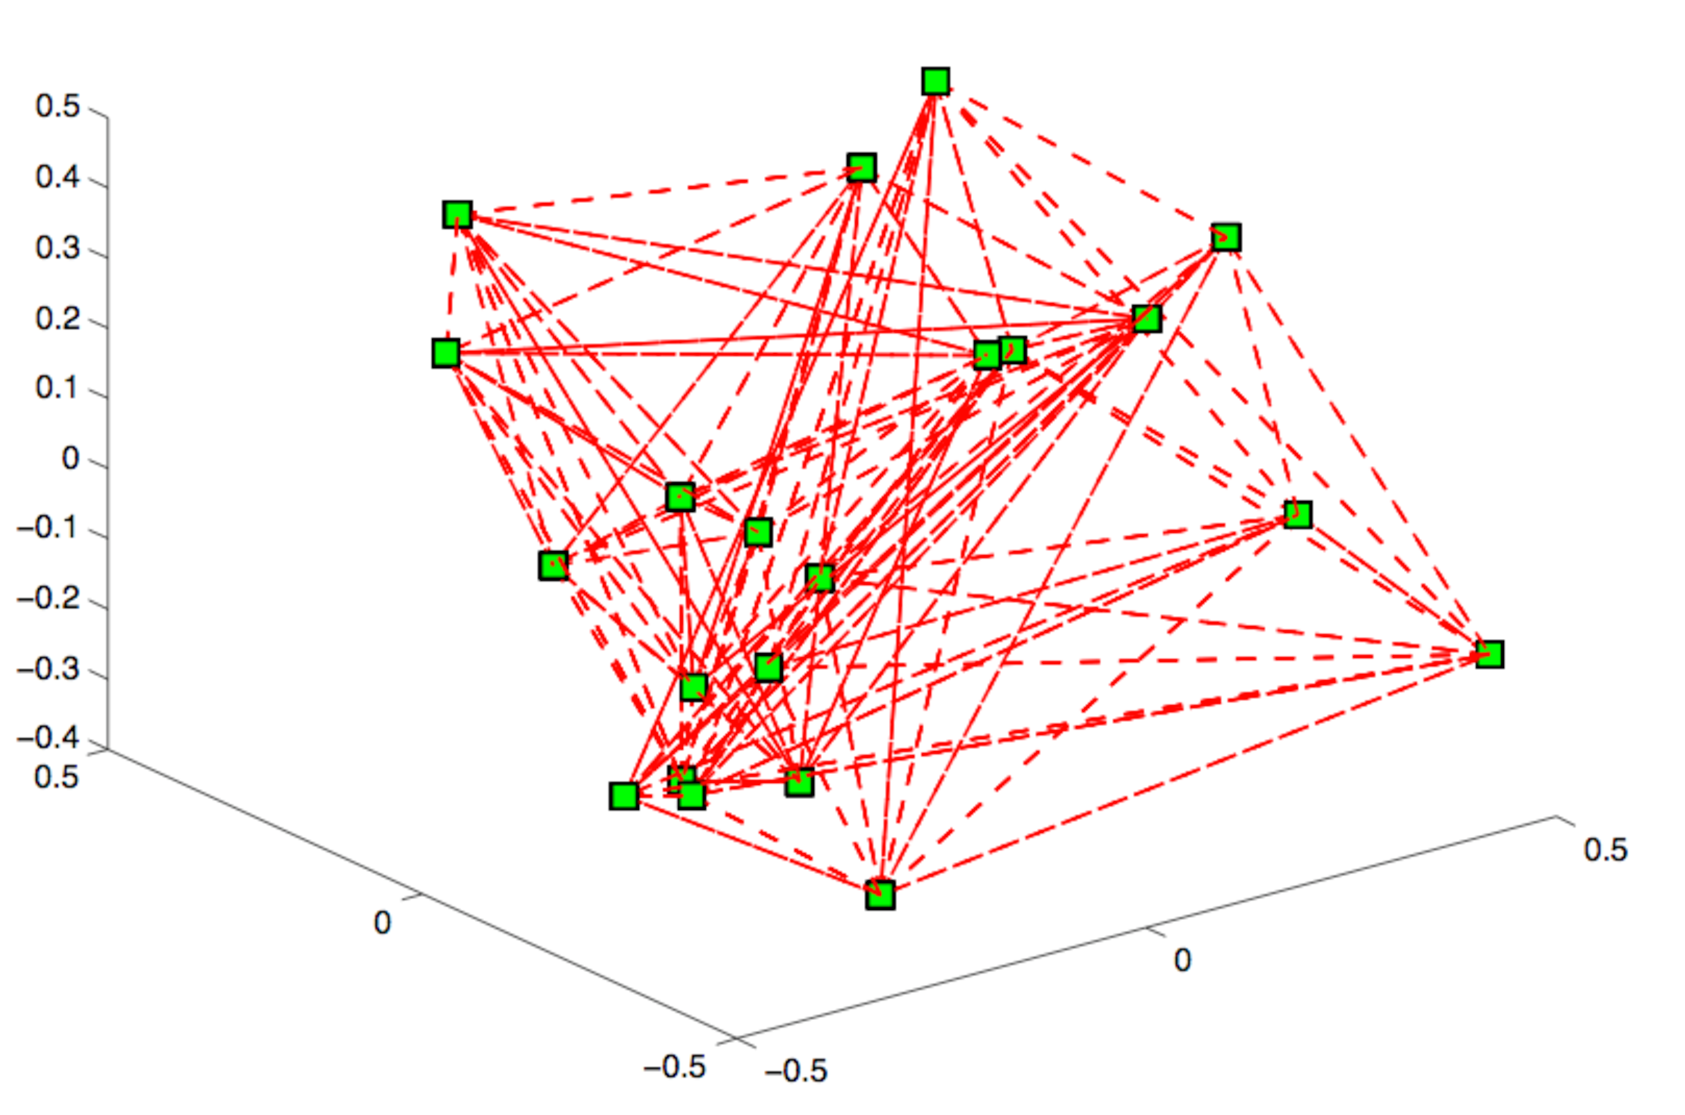
\includegraphics[height=28mm]{nbody.pdf}\\
{\scriptsize\gray{$N$-body interaction: dense, but far blocks are low rank.}}
\end{column}
\end{columns}
\vspace{1mm}
{\scriptsize\gray{Greengard \& Rokhlin, \emph{J.\ Comput.\ Phys.}\ 73 (1987); Cheng, Greengard \& Rokhlin, \emph{J.\ Comput.\ Phys.}\ 155 (1999). All FMM variants share this algorithmic skeleton; DMK departs from it.}}
\end{frame}

%================================================================
\begin{frame}{Reminder: fast Ewald as single-level kernel splitting}
\small
Recall from Part II, on the unit box:
\[
  \frac1r=\underbrace{\frac{\erf(r/\sigma)}{r}}_{M(r)\ \text{smooth}}+\underbrace{\frac{\erfc(r/\sigma)}{r}}_{R(r)\ \text{local}},\qquad
  \widehat M(\kk)=4\pi\,\frac{e^{-k^2\sigma^2/4}}{k^2}.
\]
\begin{itemize}
  \item \(M\): slowly decaying but smooth \(\Rightarrow\) few Fourier modes \(\Rightarrow\) NUFFT.
  \item \(R\): singular but numerically localized at the requested tolerance \(\Rightarrow\) direct local interactions only.
  \item \hl{Choose one \(\sigma\)} to balance both. Fine for uniform data --- but \(\sigma\) encodes \emph{one} length scale.
\end{itemize}
\begin{block}{The leap}
Instead of \emph{one} split at \emph{one} scale, telescope the kernel into a \hl{sum of splits, one per level} of an adaptive tree.
\end{block}
\end{frame}

%================================================================
\begin{frame}{Distinguishing structure of DMK}
\small
\begin{itemize}
  \item \hl{Does not use FMM-style well-separated interaction lists}; does not
  use PDE-specific expansions. Translations are generic Fourier diagonal
  scalings.
  \item \hl{Does not need a global FFT} for its \(\cO(N)\) complexity: the internal transforms have length depending only on precision, \(\cO(\log^d\tfrac1\epsilon)\), not on \(N\).
  \item \hl{Nearest-neighbor interaction list}: each box talks only to its \(3^d\) nearest neighbors (\emph{colleagues}) at each level.
  \item \hl{Dual-space}: like Ewald, uses the Fourier transform to diagonalize interactions --- but level by level, adaptively.
  \item One upward pass, one downward pass --- like the FMM.
\end{itemize}
\vspace{1mm}
\begin{block}{Slogan}
FMM-style adaptivity \(+\) Ewald-style Fourier diagonalization \(+\)
multiresolution telescoping \(=\) DMK.
\end{block}
\end{frame}

%================================================================
\begin{frame}{Roadmap of the derivation}
\small
\begin{enumerate}
  \item \textbf{Start from Ewald:} one \(\erf/\erfc\) split of \(1/r\), with a
  smooth Fourier part and a local residual.
  \item \textbf{Make it multilevel:} telescope that split into
  \(W_0+\sum_lD_l+R_L\), with one length scale per tree level.
  \item \textbf{Diagonalize each smooth difference:} \(D_l\) has a short
  plane-wave representation, so translations are diagonal scalings.
  \item \textbf{Make it adaptive and \(\cO(N)\):} tree colleagues, proxy
  interpolation, upward/downward passes, direct residuals.
  \item \textbf{PSWF kernel splittings:} Laplace, Yukawa, and the
  square-root Laplacian.
  \item \textbf{Results:} reported comparisons with FMM3D/PVFMM and the resulting algorithmic synthesis.
\end{enumerate}
\end{frame}

%----------------------------------------------------------------
\subsection{From Ewald to multilevel splitting}

\begin{frame}{From Ewald to DMK: repeat the same split}
\small
Recall the Ewald split, written with the smoothing length \(\sigma=1/\alpha\):
\[
  \frac1r=\underbrace{\frac{\erf(r/\sigma)}{r}}_{M_\sigma(r)\ \text{smooth, long range}}
  +\underbrace{\frac{\erfc(r/\sigma)}{r}}_{R_\sigma(r)\ \text{singular, local}} .
\]
\begin{itemize}
  \item \(M_\sigma\) is smooth and handled in Fourier space.
  \item \(R_\sigma\) is effectively local once
  \(\erfc(r/\sigma)\le\epsilon\) outside the neighbor region.
  \item A single \(\sigma\) is a single length scale.  That is fine for
  nearly uniform data, but not for an adaptive tree with many box sizes.
\end{itemize}
\begin{block}{DMK idea}
Use the same \(\erf/\erfc\) split on a hierarchy of length scales, not just once.
\end{block}
\end{frame}

%================================================================
\begin{frame}{Telescoping the Ewald split}
\small
Let \(\sigma_l=\sigma_0/2^l\), matched to the box size
\(\cR_l=2^{-l}\).  Since \(\erf+\erfc=1\), for any level \(L\),
\[
  \boxed{\ \frac1r
  =\frac{\erf(r/\sigma_0)}{r}
  +\sum_{l=0}^{L-1}\frac{\erf(r/\sigma_{l+1})-\erf(r/\sigma_l)}{r}
  +\frac{\erfc(r/\sigma_L)}{r}\ } .
\]
\[
  W_0(r)\approx \frac{\erf(r/\sigma_0)}{r},\qquad
  D_l(r)=\frac{\erf(r/\sigma_{l+1})-\erf(r/\sigma_l)}{r},\qquad
  R_L(r)=\frac{\erfc(r/\sigma_L)}{r}.
\]
\begin{itemize}
  \item \(W_0\): coarsest smooth piece, evaluated once.
  \item \(D_l\): level-\(l\) difference kernel, evaluated only between colleagues.
  \item \(R_L\): leaf-level residual, evaluated directly.
\end{itemize}
\end{frame}

%================================================================
\begin{frame}{Choosing the level scales}
\small
At level \(l\), choose \(\sigma_l\) so the residual is negligible outside
same-level neighboring boxes:
\[
  \erfc(r/\sigma_l)\le\epsilon
  \quad\text{for}\quad r\ge \cR_l=2^{-l},
  \qquad
  \sigma_l\approx \frac{\cR_l}{\sqrt{\log(1/\epsilon)}} .
\]
\begin{itemize}
  \item Going down one level halves the box size and halves the smoothing scale:
  \(\sigma_{l+1}=\sigma_l/2\).
  \item Interactions beyond the colleagues of a level-\(l\) box have already
  been represented by coarser pieces.
  \item Dense regions go to fine levels; sparse regions stop early.  A source
  in a coarse leaf uses the residual \(R_l\) for that coarse level.
\end{itemize}
\begin{block}{Contrast with Ewald}
Ewald uses one global \(\sigma\).  DMK uses the ladder
\(\{\sigma_l\}\), so the split scale follows the adaptive tree.
\end{block}
\end{frame}

%================================================================
\begin{frame}{The windowed coarsest piece}
\small
The coarsest smooth kernel \(\erf(r/\sigma_0)/r\) has the same \(1/k^2\)
Fourier singularity as in free-space Ewald.  Replace it by a windowed kernel
\(W_0\) whose transform is smooth at the origin:
\[
  \widehat W_0(\kk)=8\pi
  \Big(\frac{\sin(\tilde C|\kk|/2)}{|\kk|}\Big)^2
  e^{-|\kk|^2\sigma_0^2/4},
  \qquad \tilde C=\sqrt3+b\sigma_0 .
\]
\begin{itemize}
  \item \(W_0\) agrees with \(\erf(r/\sigma_0)/r\) on the physical box to
  precision \(\erfc(b)\).
  \item Its Fourier transform is smooth and rapidly decaying, so a short
  trapezoidal rule in \(\kk\) represents it spectrally.
  \item This is the same windowed-kernel construction from the fast
  free-space Ewald discussion; DMK uses it only for the coarsest piece.
\end{itemize}
\end{frame}

%----------------------------------------------------------------
\subsection{Interpolation and proxy machinery}

%================================================================
\begin{frame}{Interpolation on Chebyshev grids}
\small
A smooth function on \([-1,1]\) has a rapidly converging Chebyshev expansion
\(f(x)\approx\sum_{n=1}^p a_n T_{n-1}(x)\).
\begin{itemize}
  \item Sample at the \(p\) Chebyshev nodes \(r_i=\cos\!\big[\tfrac{\pi(p-i+1/2)}{p}\big]\); with the Vandermonde \(V(i,j)=T_{j-1}(r_i)\), coefficients are \(\bm a=V^{-1}\bm f\).
  \item Values at any other points \(\{\xi_k\}\) come from the \hl{interpolation matrix} \(U=E\,V^{-1}\), \(E(k,n)=T_{n-1}(\xi_k)\).
  \item In \(d\) dimensions: tensor-product nodes \(\rr_{\bm i}\), \(U\in\R^{q^d\times p^d}\).
\end{itemize}
\begin{block}{Band-limited error estimate (the crucial fact)}
If \(f\) is band-limited to \([-K_{\max},K_{\max}]\) and interpolated on an interval of size \(1/K_{\max}\), the error is
\(\displaystyle \cO\!\Big(\tfrac{1}{2^p p!}\Big)\|f\|_\infty\) --- rapid in \(p\), \hl{independent of \(K_{\max}\)}. This is why a fixed, small \(p\) works at every level.
\end{block}
\end{frame}

%================================================================
\begin{frame}{Anterpolation and proxy charges}
\small
For a smooth kernel \(K\), write the potential from \(N\) charges via interpolation to the Chebyshev nodes:
\[
  u(\x)=\sum_{j=1}^N \rho_j K(\x-\x_j)\approx\sum_{\bm i\in[1,p]^d}\tilde\rho_{\bm i}\,K(\x-\rr_{\bm i}),
  \qquad
  \tilde\rho_{\bm i}=\sum_{j=1}^N U^T(\bm i,j)\,\rho_j .
\]
\begin{itemize}
  \item \(U^T\) is the \hl{anterpolation matrix}; the \(\tilde\rho_{\bm i}\) are \hl{proxy charges} on a fixed \(p^d\) grid.
  \item \(N\) arbitrary sources are replaced by \(p^d\) grid sources producing the \emph{same smooth field} --- to precision \(\epsilon\).
  \item This is the DMK analog of forming a multipole expansion, but the
  construction is interpolation and is independent of the particular kernel or
  PDE.
\end{itemize}
\begin{block}{Tensor-product cost reduction}
If sources already lie on a tensor-product grid, anterpolation costs \(\cO(p^{d+1})\), not \(\cO(p^{2d})\), by separation of variables.
\end{block}
\end{frame}

%================================================================
\begin{frame}{Anterpolation cost on a tensor grid}
\small
\begin{block}{Lemma (tensor-product anterpolation)}
If the \(N\) sources lie on a \(p^d\) tensor-product Chebyshev grid, the proxy charges
\(\ \tilde\rho_{\bm i}=\sum_{\bm j} U^{T}(\bm i,\bm j)\,\rho_{\bm j}\ \)
can be formed in \(\cO(p^{d+1})\) work, not \(\cO(p^{2d})\).
\end{block}
\begin{itemize}
  \item Reason: \(U^T\) is a tensor product \(U^T=U_1^T\otimes\cdots\otimes U_d^T\); apply one factor at a time (separation of variables).
  \item This is exactly the \hl{merge} step of the upward pass: combine the \(2^d\) children's proxy grids into the parent's coarser grid.
  \item The same tensor-product factorization reduces every ``grid \(\to\) grid'' map in DMK from \(p^{2d}\) to \(p^{d+1}\).
\end{itemize}
\end{frame}

%================================================================
\begin{frame}{Shifting a Chebyshev expansion to a child}
\small
\begin{block}{Lemma (parent \(\to\) child)}
A tensor Chebyshev polynomial on box \(B\), \(\ u(\x)=\sum_{\bm n}\alpha_{\bm n}T_{\bm n-\bm1}(\x)\), equals, on a child \(C\subset B\), \(\ u(\x)=\sum_{\bm n'}\beta_{\bm n'}T'_{\bm n'-\bm1}(\x)\) with
\(\ \beta=V^{-1}E\,\alpha\), computable in \(\cO(p^{d+1})\).
\end{block}
\begin{itemize}
  \item The translation is \hl{exact} --- we only re-center and re-scale a polynomial.
  \item This is the \hl{split} step of the downward pass: pass the incoming (smooth) field from a parent to its children before touching targets.
  \item Together with anterpolation, these two lemmas are the entire ``fine-to-coarse'' and ``coarse-to-fine'' machinery --- pure interpolation, no kernel.
\end{itemize}
\end{frame}

%================================================================
\begin{frame}{Fourier tools}
\small
Conventions and the two facts we lean on:
\[
  \widehat F(\kk)=\int e^{-\ii\kk\cdot\x}F(\x)\dd\x,\qquad
  F(\x)=\frac{1}{(2\pi)^d}\int e^{\ii\kk\cdot\x}\widehat F(\kk)\dd\kk .
\]
\begin{itemize}
  \item \hl{Duality.} With the required integrability, spatial smoothness yields Fourier decay, while Fourier smoothness yields spatial decay. The construction exploits this complementary behavior.
  \item \hl{Poisson summation.} \(\displaystyle\sum_n f\!\big(x+\tfrac{2\pi n}{h}\big)=\tfrac{h}{2\pi}\sum_m \widehat f(mh)e^{\ii mhx}\): governs the aliasing error of the trapezoidal rule, as in the NUFFT analysis.
\end{itemize}
\begin{block}{Design principle for DMK}
Every kernel piece is constructed to be rapidly decaying in the representation
used for its evaluation, to the requested tolerance: Fourier space for smooth
pieces and physical space for residual pieces. \hl{Dual-space.}
\end{block}
\end{frame}

%----------------------------------------------------------------
\subsection{Multilevel kernel splitting}

%================================================================
\begin{frame}{The mollified far kernel at each level}
\small
Define the level-\(L\) \hl{mollified far kernel}
\[
  M_L(r)=\frac{\erf(r/\sigma_L)}{r}=M_0(r)+\sum_{l=0}^{L-1}D_l(r).
\]
\begin{itemize}
  \item \(M_L\) accounts, to precision \(\epsilon\), for \emph{all} interactions \hl{beyond the colleagues} of a box at level \(L\).
  \item The remaining correction is \(R_L\), confined to colleagues and coarse neighbors.
  \item Reading the telescope forward: each new level \(l\) adds one difference kernel \(D_l\), sharpening \(M_l\to M_{l+1}\) as the boxes shrink.
  \item At level \(L=1\) the colleagues already cover the whole domain --- \(M_0\) (windowed) is the only global piece.
\end{itemize}
\end{frame}

%================================================================
\begin{frame}{The dual-space picture}
\small
In \hl{physical space} the split is
\[
  \frac1r\approx W_0(r)+\frac{\erf(r/\sigma_1)-\erf(r/\sigma_0)}{r}+\cdots+\frac{\erfc(r/\sigma_L)}{r}.
\]
In \hl{Fourier space} (using \(\widehat{1/r}=4\pi/k^2\)) the same identity reads
\[
  \frac{4\pi}{k^2}\approx \widehat W_0(\kk)
  +\underbrace{4\pi\,\frac{e^{-k^2\sigma_1^2/4}-e^{-k^2\sigma_0^2/4}}{k^2}}_{\widehat D_0}+\cdots
  +4\pi\,\frac{1-e^{-k^2\sigma_L^2/4}}{k^2}.
\]
\begin{itemize}
  \item Each difference kernel is effectively localized in physical space and rapidly decaying in Fourier space at the requested tolerance.
  \item That double locality is why each level costs \(\cO(N)\) and needs only a short transform.
\end{itemize}
\end{frame}

%================================================================
\begin{frame}{Kernel split pieces for \(1/r\)}
\small
\begin{columns}[T,totalwidth=\textwidth]
\begin{column}{0.5\textwidth}
\centering
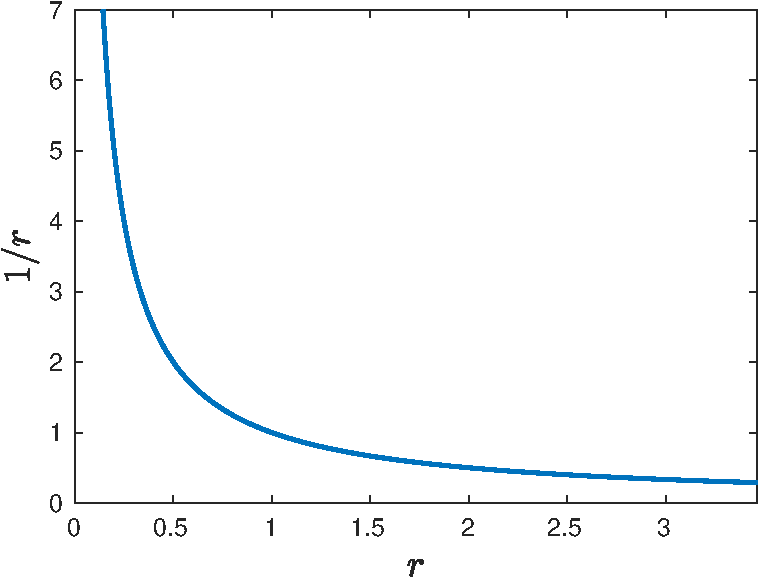
\includegraphics[height=30mm]{l3dkernelsplit1a.pdf}\\
{\scriptsize the original kernel \(1/r\)}
\end{column}
\begin{column}{0.5\textwidth}
\centering
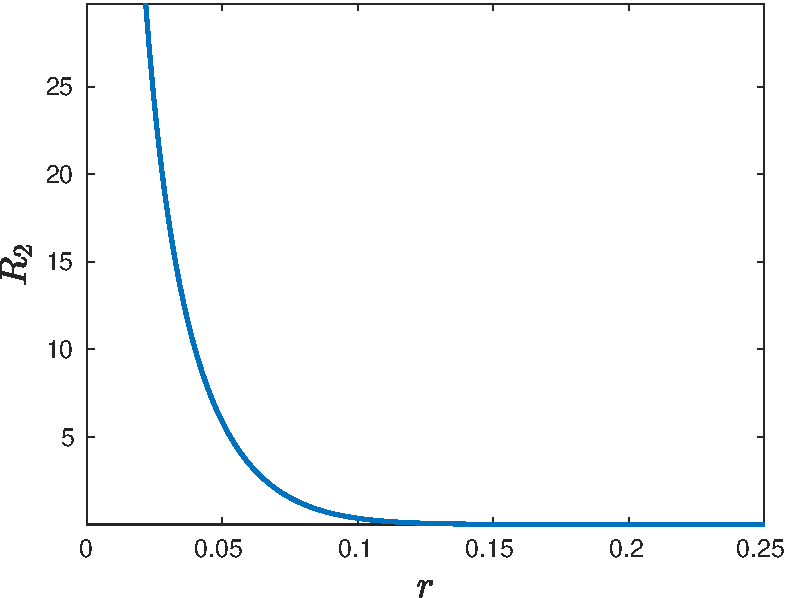
\includegraphics[height=30mm]{l3dkernelsplit1b.pdf}\\
{\scriptsize residual \(R_2(r)\): numerically supported on \([0,\tfrac14]\)}
\end{column}
\end{columns}
\vspace{2mm}
{\scriptsize\gray{Dual-space splitting of \(1/r\) on a level-2 leaf box, six digits: \(1/r=W_0+D_0+D_1+R_2\) for \(r\le\sqrt3\). The residual is numerically localized and handled directly.}}
\end{frame}

%================================================================
\begin{frame}{Windowed kernel and Fourier transform}
\small
\begin{columns}[T,totalwidth=\textwidth]
\begin{column}{0.5\textwidth}
\centering
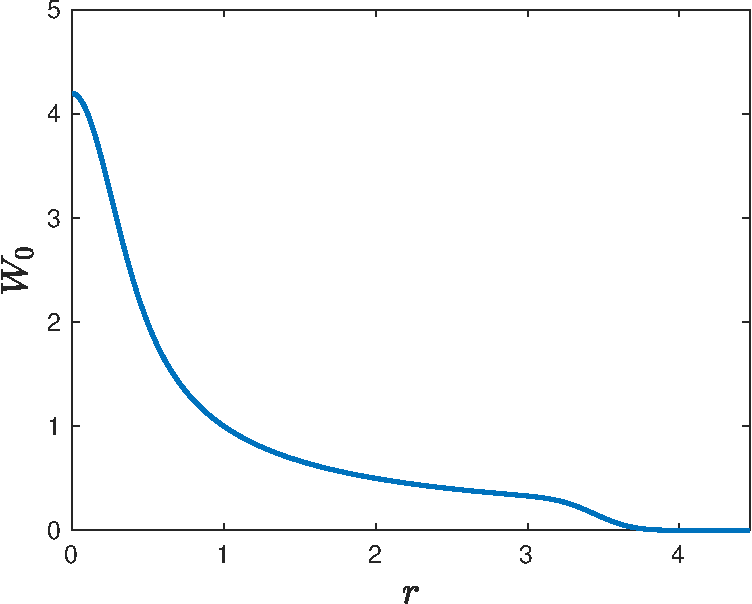
\includegraphics[height=30mm]{l3dkernelsplit2a.pdf}\\
{\scriptsize windowed kernel \(W_0(r)\): smooth, long-range}
\end{column}
\begin{column}{0.5\textwidth}
\centering
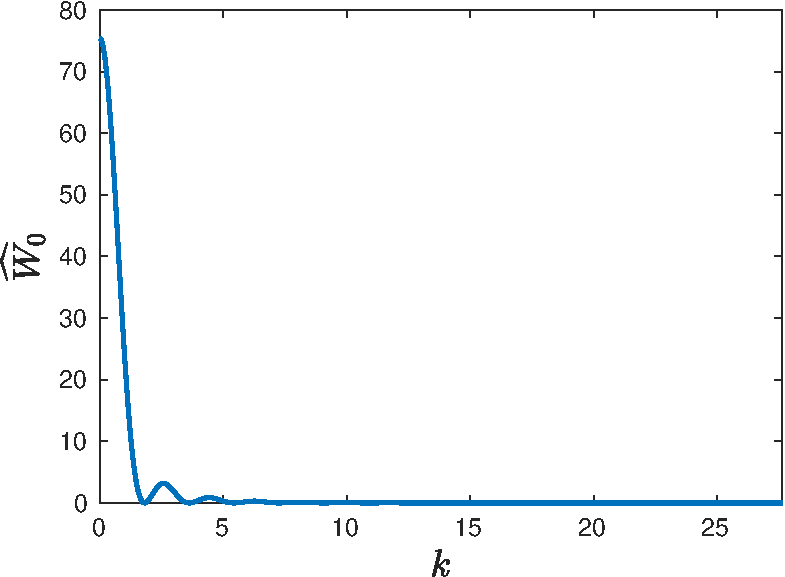
\includegraphics[height=30mm]{l3dkernelsplit2b.pdf}\\
{\scriptsize \(\widehat W_0(\kk)\): smooth at the origin, fast decay}
\end{column}
\end{columns}
\vspace{2mm}
The windowed kernel removes the \(1/k^2\) singularity exactly as in Part II:
\[
  \widehat W_0(\kk)=8\pi\Big(\frac{\sin(\tilde C|\kk|/2)}{|\kk|}\Big)^2 e^{-|\kk|^2\sigma_0^2/4},\quad \tilde C=\sqrt3+b\sigma_0,
\]
with \(|W_0(r)-M_0(r)|\le \epsilon/r\) for \(r\le\sqrt3\) when \(\erfc(b)\le\epsilon\) (for example, \(b=6\) gives more than 15 digits).
\end{frame}

%================================================================
\begin{frame}{Self-similarity of difference kernels}
\small
\begin{columns}[T,totalwidth=\textwidth]
\begin{column}{0.5\textwidth}
\centering
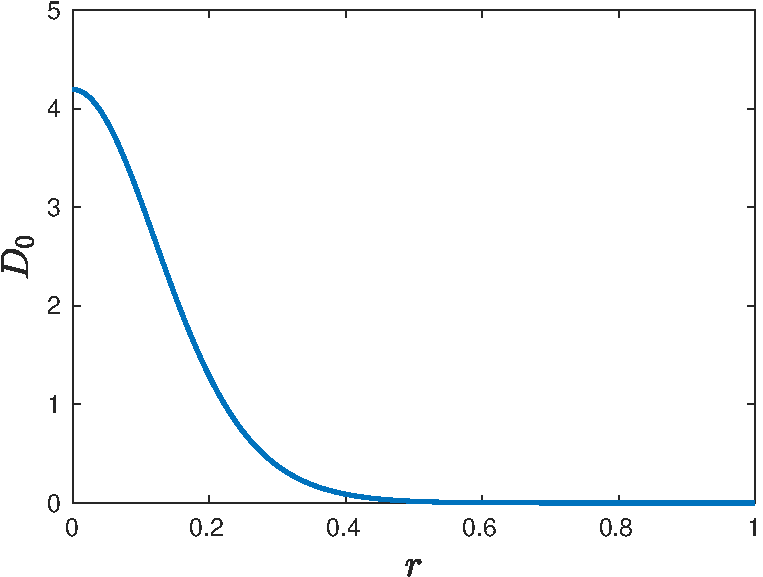
\includegraphics[height=27mm]{l3dkernelsplit3a.pdf}\\
{\scriptsize \(D_0(r)\), numerically localized on \([0,1]\), and its transform}
\end{column}
\begin{column}{0.5\textwidth}
\centering
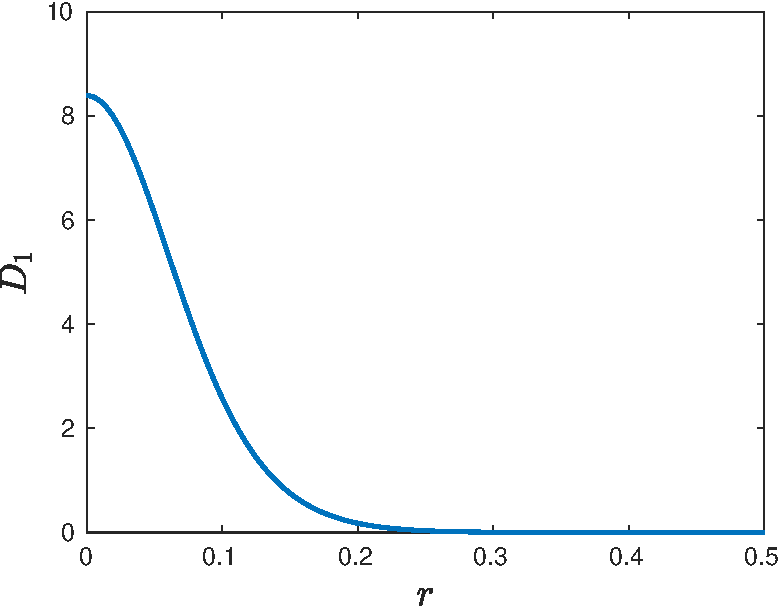
\includegraphics[height=27mm]{l3dkernelsplit4a.pdf}\\
{\scriptsize \(D_1(r)\), numerically localized on \([0,\tfrac12]\), and its transform}
\end{column}
\end{columns}
\vspace{2mm}
\begin{block}{Key structural fact}
\(D_1\) is exactly a \hl{rescaled copy} of \(D_0\): half the support, twice the frequency content. Going down one level \emph{halves the length scale but doubles the bandwidth} --- so the number of Fourier modes stays \hl{constant across levels}.
\end{block}
\end{frame}

%================================================================
\begin{frame}{The difference-kernel Fourier transform}
\small
\[
  \widehat D_l(\kk)=
  \begin{cases}
    4\pi\,\dfrac{e^{-|\kk|^2\sigma_{l+1}^2/4}-e^{-|\kk|^2\sigma_l^2/4}}{|\kk|^2}, & \kk\neq\bm0,\\[8pt]
    \pi(\sigma_l^2-\sigma_{l+1}^2), & \kk=\bm0.
  \end{cases}
\]
\begin{itemize}
  \item Perfectly \hl{smooth} (no singularity at \(\kk=\bm0\): the numerator vanishes like \(k^2\)).
  \item \hl{Rapidly decaying} (the \(e^{-k^2\sigma_{l+1}^2/4}\) factor).
  \item Smooth \(+\) fast-decaying \(\Rightarrow\) the trapezoidal rule in \(\kk\) converges \hl{exponentially}. A short sum represents \(D_l\) to precision \(\epsilon\).
\end{itemize}
\begin{block}{Residual}
\(R_L(r)\) is numerically localized: \(\ |R_L(r)|\le \epsilon/r\) for \(r\ge\cR_L\). It is evaluated only by local direct sums.
\end{block}
\end{frame}

%----------------------------------------------------------------
\subsection{Fourier machinery and diagonal translation}

\begin{frame}{From a smooth Fourier kernel to a short plane-wave sum}
\small
Truncating and discretizing the inverse Fourier transform of \(\widehat D_l\) gives
\[
  D_l(\x)\approx\sum_{\mm\in[-n_f,n_f]^d} w_{l,\mm}\,e^{\ii h_l\,\mm\cdot\x},\qquad
  w_{l,\mm}=\frac{h_l^d}{(2\pi)^d}\,\widehat D_l(h_l\mm).
\]
\begin{itemize}
  \item The number of modes \(N_F=(2n_f+1)^d\) is independent of the level \(l\) and of \(N\), once the requested precision is fixed.
  \item The precision-dependent values are determined by the split and quadrature; Table 1 later gives the PSWF values used for 3D Laplace DMK.
  \item This is why DMK \hl{does not need a global FFT}: the transforms are short enough to apply directly.
\end{itemize}
\end{frame}

%================================================================
\begin{frame}{Level-independent plane-wave mode count}
\small
The difference kernel \(D_l\) lives on scale \(\cR_l\); decreasing the physical scale increases its Fourier bandwidth by the reciprocal factor.
\begin{itemize}
  \item Going from level \(l\) to \(l+1\): \(\sigma\) halves, so the Fourier range \(K_l\) \hl{doubles}.
  \item But the relevant source--target distances \hl{also halve} --- the number of oscillations across a box is unchanged.
  \item Net: the number of trapezoidal nodes is \hl{level-independent} at fixed precision.
\end{itemize}
\begin{block}{Consequence}
Because \(N_F\) depends only on \(\epsilon\), each level's Fourier work is \(\cO(1)\) per box. \hl{No global FFT is needed} for \(\cO(N)\); the transforms are short enough to apply directly.
\end{block}
\end{frame}

%================================================================
\begin{frame}{Period selection and aliasing}
\small
\begin{columns}[T,totalwidth=\textwidth]
\begin{column}{0.56\textwidth}
\begin{itemize}
  \item \(D_l\) is localized (to \(\epsilon\)) on a ball of radius \(\cR_l\).
  \item But we must evaluate it for source--target pairs within \emph{colleagues}: distances up to \(2\cR_l\).
  \item The trapezoidal rule periodizes \(D_l\). Its period is selected so that images stay outside the colleague region at the requested tolerance.
\end{itemize}
\end{column}
\begin{column}{0.42\textwidth}
\centering
\begin{tikzpicture}[scale=0.85]
  \draw[->](-2.6,0)--(2.6,0) node[right]{\scriptsize $r$};
  \draw[thick,CCMorange] plot[smooth,domain=-1:1,samples=40]({\x},{1.4*exp(-6*\x*\x)});
  \draw[<->,SFdark] (-1,-0.25)--(1,-0.25) node[midway,below]{\scriptsize supp $=2\cR_l$};
  \draw[<->,mygray] (-1.5,1.5)--(1.5,1.5) node[midway,above]{\scriptsize colleague evaluation region};
  \draw[dashed,mygray] (-1.5,0)--(-1.5,1.5);\draw[dashed,mygray](1.5,0)--(1.5,1.5);
\end{tikzpicture}
\end{column}
\end{columns}
\end{frame}

%================================================================
\begin{frame}{Outgoing and incoming plane-wave expansions}
\small
For a box \(B\) at level \(l\) with center \(\cc(B)\), define the \hl{outgoing expansion} (a type-1 sum over its sources)
\[
  [\Phi_l(B)]_{\mm}=\sum_{\y_j\in B} e^{-\ii h_l\mm\cdot(\y_j-\cc(B))}\rho_j,\qquad \mm\in[-n_f,n_f]^d .
\]
The difference-kernel field at a target \(\x_i\in B\) from all colleagues is the \hl{incoming expansion}
\[
  u_l^{\rm diff}(\x_i)=\sum_{\mm} e^{\ii h_l\mm\cdot(\x_i-\cc(B))}\,[\Psi_l(B)]_{\mm},
\]
where \([\Psi_l(B)]_{\mm}=\displaystyle\sum_{S\in C(B)} w_{l,\mm}\,e^{\ii h_l\mm\cdot(\cc(B)-\cc(S))}\,[\Phi_l(S)]_{\mm}.\)
\begin{itemize}
  \item These sums have the algebraic form of type-1/type-2 Fourier sums, but
  in DMK \(N_F\) is small enough that they are usually evaluated directly.
\end{itemize}
\end{frame}

%================================================================
\begin{frame}{Diagonal translation in plane-wave form}
\small
Because the representation is in \hl{pure exponentials}, translating an
outgoing expansion in box \(S\) to an incoming expansion in box \(B\) reduces
to multiplication mode-by-mode:
\[
  [\Psi_l(B)]_{\mm}=\sum_{S\in C(B)} \underbrace{w_{l,\mm}\,e^{\ii h_l\mm\cdot(\cc(B)-\cc(S))}}_{\text{scalar, per mode}}\ [\Phi_l(S)]_{\mm}.
\]
\begin{itemize}
  \item No dense \hl{M2L} matrix as in the FMM --- the ``translation operator'' is \hl{diagonal}.
  \item Each box interacts only with its \(\le 3^d\) colleagues; cost \(\cO(3^d N_F)\) per box.
  \item The translation machinery is \emph{kernel-independent}: only the weights \(w_{l,\mm}=\tfrac{h_l^d}{(2\pi)^d}\widehat D_l(h_l\mm)\) depend on the kernel being evaluated.
\end{itemize}
\begin{block}{This is the ``dual-space'' payoff}
Physical-space translation \(\to\) Fourier-space diagonal scaling. Exactly Ewald's diagonalization, but applied \emph{per level}.
\end{block}
\end{frame}

%================================================================
\begin{frame}{Interaction lists: DMK vs.\ FMM}
\small
\begin{columns}[T,totalwidth=\textwidth]
\begin{column}{0.5\textwidth}
\centering
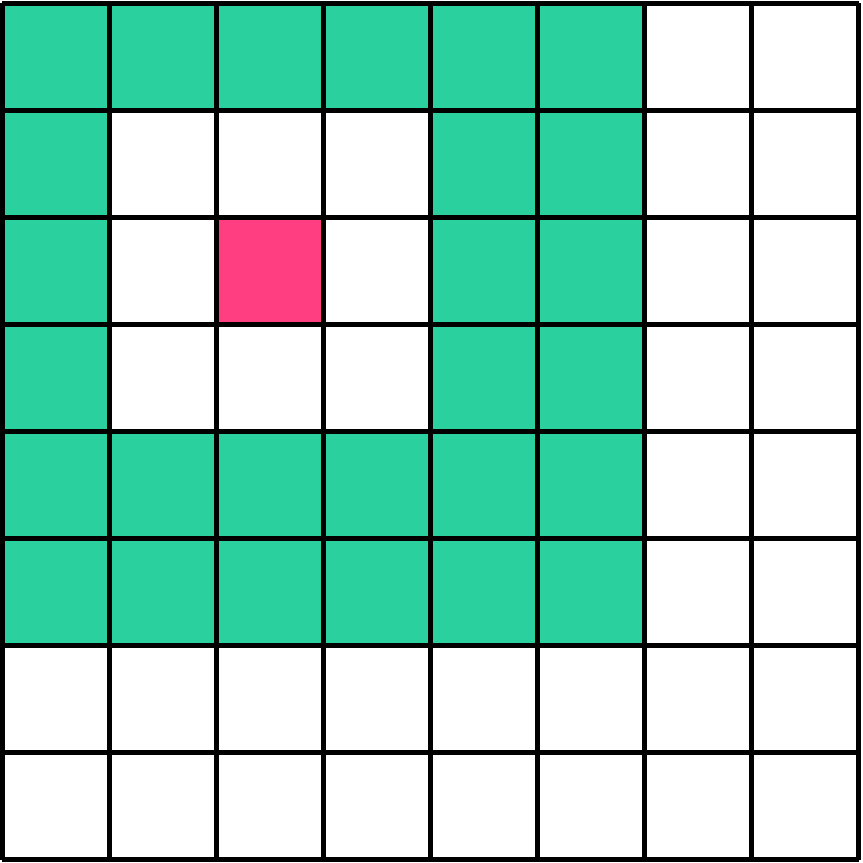
\includegraphics[height=34mm]{fmminteractionlist.pdf}\\
{\scriptsize FMM: up to \(6^d-3^d=189\) boxes (3D)}
\end{column}
\begin{column}{0.5\textwidth}
\centering
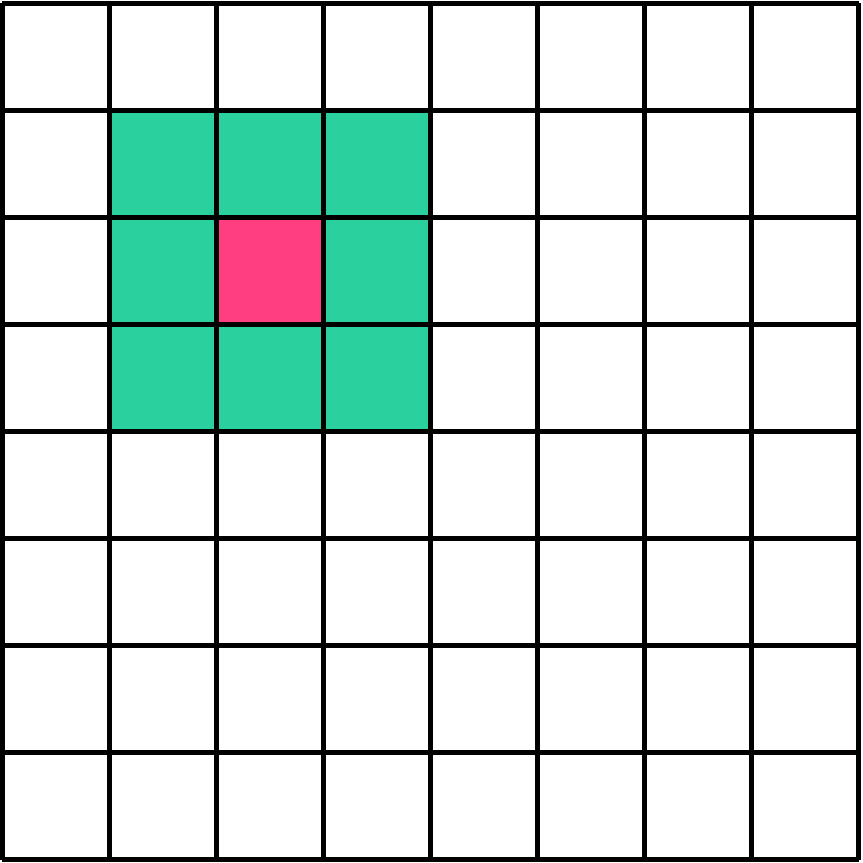
\includegraphics[height=34mm]{dmkinteractionlist.pdf}\\
{\scriptsize DMK: only same-level adjacent boxes, called colleagues (\(3^d=27\) in 3D)}
\end{column}
\end{columns}
\vspace{1mm}
\begin{itemize}
  \item FMM separates near/far, so it needs the ``interaction list'' of well-separated boxes.
  \item DMK does not form a separate well-separated interaction list: at each level it convolves \(D_l\) only with same-level nearest neighbors. Interactions beyond these neighbors are represented at coarser levels.
\end{itemize}
\end{frame}

%----------------------------------------------------------------
\subsection{The adaptive algorithm}

\begin{frame}{The adaptive tree: colleagues and neighbors}
\small
\begin{columns}[T,totalwidth=\textwidth]
\begin{column}{0.52\textwidth}
\begin{itemize}
  \item \hl{Level-restricted} tree: neighboring leaves differ by \(\le1\) level.
  \item \hl{Colleagues} of \(B\): same-level boxes sharing a boundary point (incl.\ \(B\)); \(\le 3^d\).
  \item \hl{Coarse neighbors} \(\cN(B)\): adjacent leaves one level up.
  \item Refine until each leaf has \(\le n_s\) points; \(n_s\) is selected to balance local work against the remaining algorithmic work.
\end{itemize}
\end{column}
\begin{column}{0.46\textwidth}
\centering
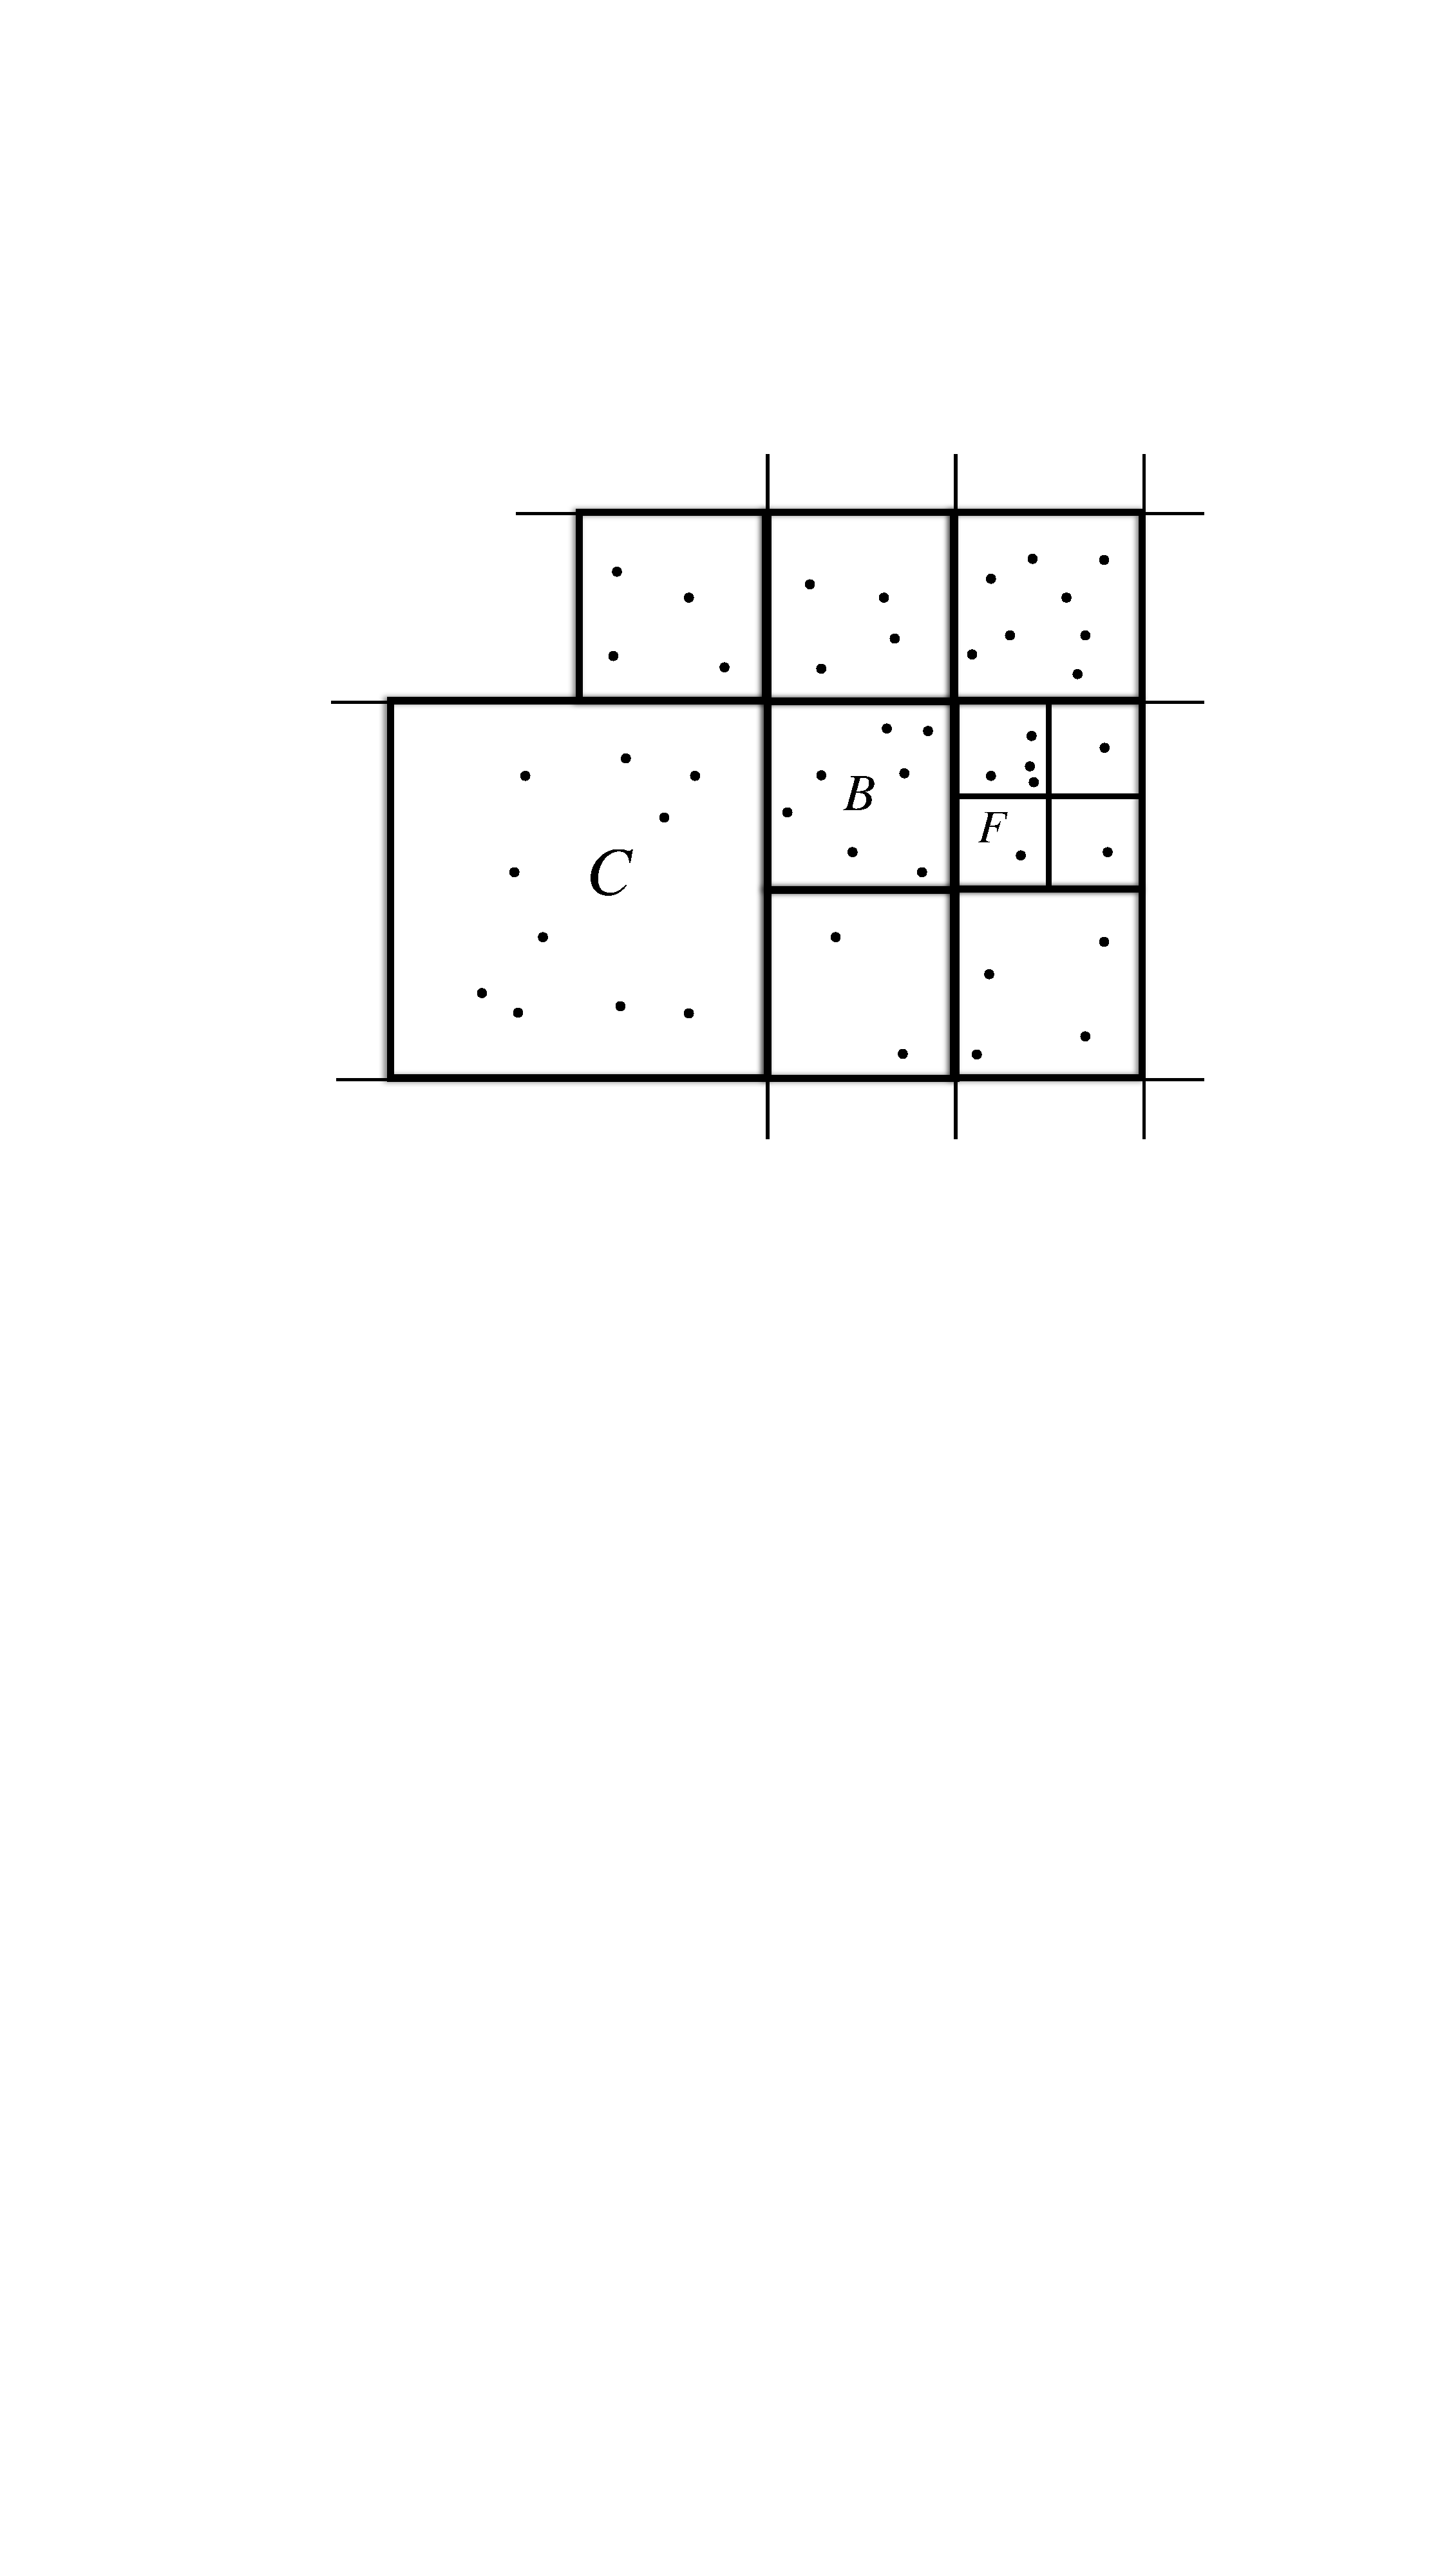
\includegraphics[height=34mm]{dmk_boxdefs.pdf}\\
{\scriptsize\gray{Leaf \(B\); \(F\) fine neighbor, \(C\) coarse neighbor.}}
\end{column}
\end{columns}
\end{frame}

%================================================================
\begin{frame}{The adaptive tree in action}
\small
\begin{columns}[T,totalwidth=\textwidth]
\begin{column}{0.5\textwidth}
\centering
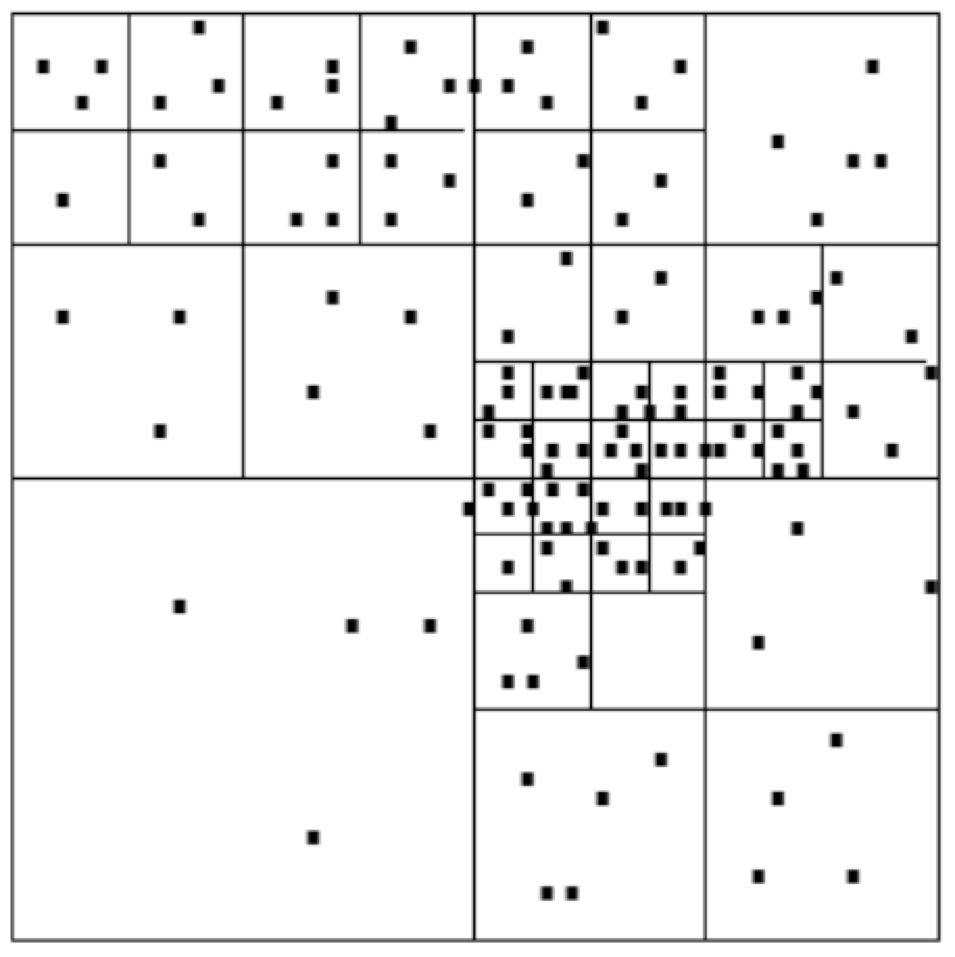
\includegraphics[height=40mm]{adaptivetree.png}
\end{column}
\begin{column}{0.5\textwidth}
\begin{itemize}
  \item Refinement follows the data: dense regions get deep trees, empty regions stay coarse.
  \item Each source lives in \emph{some} leaf at \emph{some} level; its residual \(R_l\) reaches only that leaf's colleagues.
  \item A source in a coarse leaf (e.g.\ \(\y'\) at level 3) uses \(R_3\) --- adaptivity is automatic once the telescoping ladder \(\{\sigma_l\}\) is in place.
\end{itemize}
\end{column}
\end{columns}
\end{frame}

%================================================================
\begin{frame}{First version: the \(\cO(N\log N)\) algorithm}
\small
Using \(u(\x_i)=u^{\rm win}(\x_i)+\sum_{l}u_l^{\rm diff}(\x_i)+u_L^{\rm local}(\x_i)\):
\begin{enumerate}\itemsep2pt
  \item Sort sources/targets into a level-restricted adaptive tree.
  \item \textbf{Windowed (level 0):} evaluate \(u^{\rm win}=\sum_j W_0(\x_i-\y_j)\rho_j\) globally via a short plane-wave sum, \(N_F\) independent of \(N\).
  \item \textbf{Difference (each level \(l\)):} form outgoing \(\Phi_l(B)\), diagonally translate to incoming \(\Psi_l(B)\) over colleagues, evaluate \(u_l^{\rm diff}\).
  \item \textbf{Local (leaves):} add \(R_l(\x_i-\y_j)\rho_j\) directly over colleagues / coarse neighbors.
\end{enumerate}
\begin{block}{Why \(\cO(N\log N)\)}
\(\cO(N)\) work at each of \(\cO(\log N)\) levels because we touch every source and target \emph{at every level}. Next: remove that redundancy.
\end{block}
\end{frame}

%================================================================
\begin{frame}{Toward \(\cO(N)\): proxy charges and two passes}
\small
The inefficiency above is re-accessing all points at every level. DMK removes it as in the FMM, but with \hl{interpolation instead of expansions}.
\begin{center}
\begin{tikzpicture}[scale=0.9]
  \draw[thick] (0,0) rectangle (3,3);
  \draw (1.5,0)--(1.5,3); \draw (0,1.5)--(3,1.5);
  \foreach \a/\b in {0.3/0.4,0.7/0.6,2.2/0.5,2.6/2.4,0.6/2.5,2.4/0.7,0.4/2.2}
     \fill[SFdark] (\a,\b) circle (1pt);
  \foreach \dx/\dy in {0/0,1.5/0,0/1.5,1.5/1.5}
    \foreach \x in {0.42,0.75,1.08}
      \foreach \y in {0.42,0.75,1.08}
        \fill[CCMorange] (\dx+\x,\dy+\y) circle (1.1pt);
  \draw[->,thick,CCMorange] (3.4,1.5)--(4.4,1.5) node[midway,above]{\scriptsize anterp};
  \draw[thick] (4.8,0.75) rectangle (6.3,2.25);
  \foreach \x/\y in {5.15/1.10,5.55/1.10,5.95/1.10,
                        5.15/1.50,5.55/1.50,5.95/1.50,
                        5.15/1.90,5.55/1.90,5.95/1.90}
     \fill[CCMorange] (\x,\y) circle (1.3pt);
  \node[align=center] at (5.55,-0.1){\scriptsize parent proxy grid};
  \node[align=center] at (1.5,-0.4){\scriptsize children: sources $\to$ proxy grids};
\end{tikzpicture}
\end{center}
\begin{itemize}
  \item \hl{Upward pass:} at leaves, anterpolate sources to \(p^d\) proxy charges; merge children's proxies into the parent's (tensor-product, \(\cO(p^{d+1})\)).
  \item \hl{Downward pass:} convert incoming plane waves to a Chebyshev expansion, split from parent to children, evaluate at leaves only.
\end{itemize}
\end{frame}

%================================================================
\begin{frame}{The upward pass}
\small
\begin{center}
\begin{tikzpicture}[>=Latex,scale=0.9,transform shape,node distance=6mm]
  \node[draw,rounded corners=2pt,fill=black!4,inner sep=5pt,align=center] (a){sources in\\leaf box};
  \node[draw,rounded corners=2pt,fill=CCMorange!15,inner sep=5pt,align=center,right=10mm of a] (b){proxy charges\\(anterpolation, $U^T$)};
  \node[draw,rounded corners=2pt,fill=CCMorange!15,inner sep=5pt,align=center,right=10mm of b] (c){parent proxies\\(merge children)};
  \draw[->,thick,CCMorange](a)--node[above]{\scriptsize $\cO(p^dN)$}(b);
  \draw[->,thick,CCMorange](b)--node[above]{\scriptsize $\cO(p^{d+1}N_B)$}(c);
\end{tikzpicture}
\end{center}
\begin{itemize}
  \item At each leaf: replace the (up to \(n_s\)) sources by \(p^d\) proxy charges on a Chebyshev grid that reproduce the same smooth far field.
  \item Merge: the \(2^d\) children's proxy grids are anterpolated onto the parent's coarser grid --- pure interpolation, tensor-product, \(\cO(p^{d+1})\) per box.
  \item After the upward pass, every non-leaf box carries a small set of proxy charges; later levels use these compressed data rather than the original sources.
\end{itemize}
\end{frame}

%================================================================
\begin{frame}{The downward pass}
\small
\begin{center}
\begin{tikzpicture}[>=Latex,scale=0.86,transform shape,node distance=5mm]
  \node[draw,rounded corners=2pt,fill=black!4,inner sep=4pt,align=center] (a){proxy charges\\$\to$ outgoing PW $\Phi_l$};
  \node[draw,rounded corners=2pt,fill=CCMorange!15,inner sep=4pt,align=center,right=8mm of a] (b){diagonal translate\\$\Phi_l\!\to\!\Psi_l$ (colleagues)};
  \node[draw,rounded corners=2pt,fill=black!4,inner sep=4pt,align=center,right=8mm of b] (c){incoming PW\\$\to$ proxy potential};
  \node[draw,rounded corners=2pt,fill=CCMorange!15,inner sep=4pt,align=center,below=6mm of c] (d){split parent\\$\to$ children (interp)};
  \node[draw,rounded corners=2pt,fill=black!4,inner sep=4pt,align=center,left=8mm of d] (e){evaluate at\\targets in leaves};
  \draw[->,thick,CCMorange](a)--(b);\draw[->,thick,CCMorange](b)--(c);
  \draw[->,thick,CCMorange](c)--(d);\draw[->,thick,CCMorange](d)--(e);
\end{tikzpicture}
\end{center}
\begin{itemize}
  \item Form outgoing plane waves from proxy charges; diagonally translate to incoming plane waves over colleagues (the level-\(l\) difference-kernel interaction).
  \item Convert the incoming plane-wave field to a Chebyshev expansion; \hl{interpolate parent \(\to\) children} recursively.
  \item Only at a leaf do we evaluate at the actual targets. \hl{Each target is touched once.}
\end{itemize}
\end{frame}

%================================================================
\begin{frame}{The local (direct) interactions}
\small
The residual kernel \(R_l\) is numerically localized, so at the finest relevant level each source contributes directly to nearby targets only:
\[
  u(\x_i)\mathrel{+}=\sum_{\y_j\in \text{colleagues}\,\cup\,\cN(B)} R_l(\x_i-\y_j)\,\rho_j .
\]
\begin{itemize}
  \item The colleague and coarse-neighbor lists bound the direct work for a level-restricted tree at fixed leaf occupancy.
  \item The local kernel is evaluated only where its magnitude exceeds the requested tolerance.
  \item When sources and targets coincide, the diagonal is handled according to the underlying kernel and problem formulation.
\end{itemize}
\end{frame}

%================================================================
\begin{frame}{Putting it together: the \(\cO(N)\) cost count}
\small
\begin{tabular}{@{}lll@{}}
\toprule
Pass & Step & Cost \\
\midrule
Upward & sources \(\to\) leaf proxy charges & \(\cO(p^d N)\)\\
       & merge children \(\to\) parent proxies & \(\cO(p^{d+1} N_B)\)\\
\addlinespace
Downward & proxy \(\to\) outgoing plane waves & \(\cO(p\,n_f^d N_B)\)\\
         & diagonal translation (colleagues) & \(\cO(3^d n_f^d N_B)\)\\
         & incoming \(\to\) proxy potential & \(\cO(p\,n_f^d N_B)\)\\
         & split parent \(\to\) children & \(\cO(p^{d+1} N_B)\)\\
         & proxy potential \(\to\) targets & \(\cO(p^d N)\)\\
\addlinespace
Direct & local residual interactions & \(\cO(n_s N)\)\\
\bottomrule
\end{tabular}
\par\smallskip
\noindent For a level-restricted adaptive tree with fixed \(n_s\), \(N_B=\cO(N/n_s)\). With \(p\) and \(n_f\) fixed by \(\epsilon\), every displayed term is \(\cO(N)\). The two passes avoid a factor of \(\log N\) by touching physical sources and targets only at the leaves.
\end{frame}

%================================================================
\begin{frame}{Work count for adaptive \(\cO(N)\) summation}
\small
\begin{itemize}
  \item The residual is evaluated only across local colleague and coarse-neighbor lists, with negligible tails omitted at the requested tolerance.
  \item For a level-restricted tree with fixed leaf occupancy, the total direct work is \(\cO(N)\).
  \item The constants depend on the local cutoff, the leaf occupancy, and the geometry of the distribution.
\end{itemize}
\begin{block}{Level count}
With \(L_{\max}=\cO(\log N)\) levels but only \(\cO(1)\) work per box per level (fixed \(p\), \(n_f\)), and \(N_B=\cO(N/n_s)\) boxes in a level-restricted tree, the two passes are \(\cO(N)\) --- no \(\log N\).
\end{block}
\end{frame}

%================================================================
\begin{frame}{The DMK framework}
\begin{center}
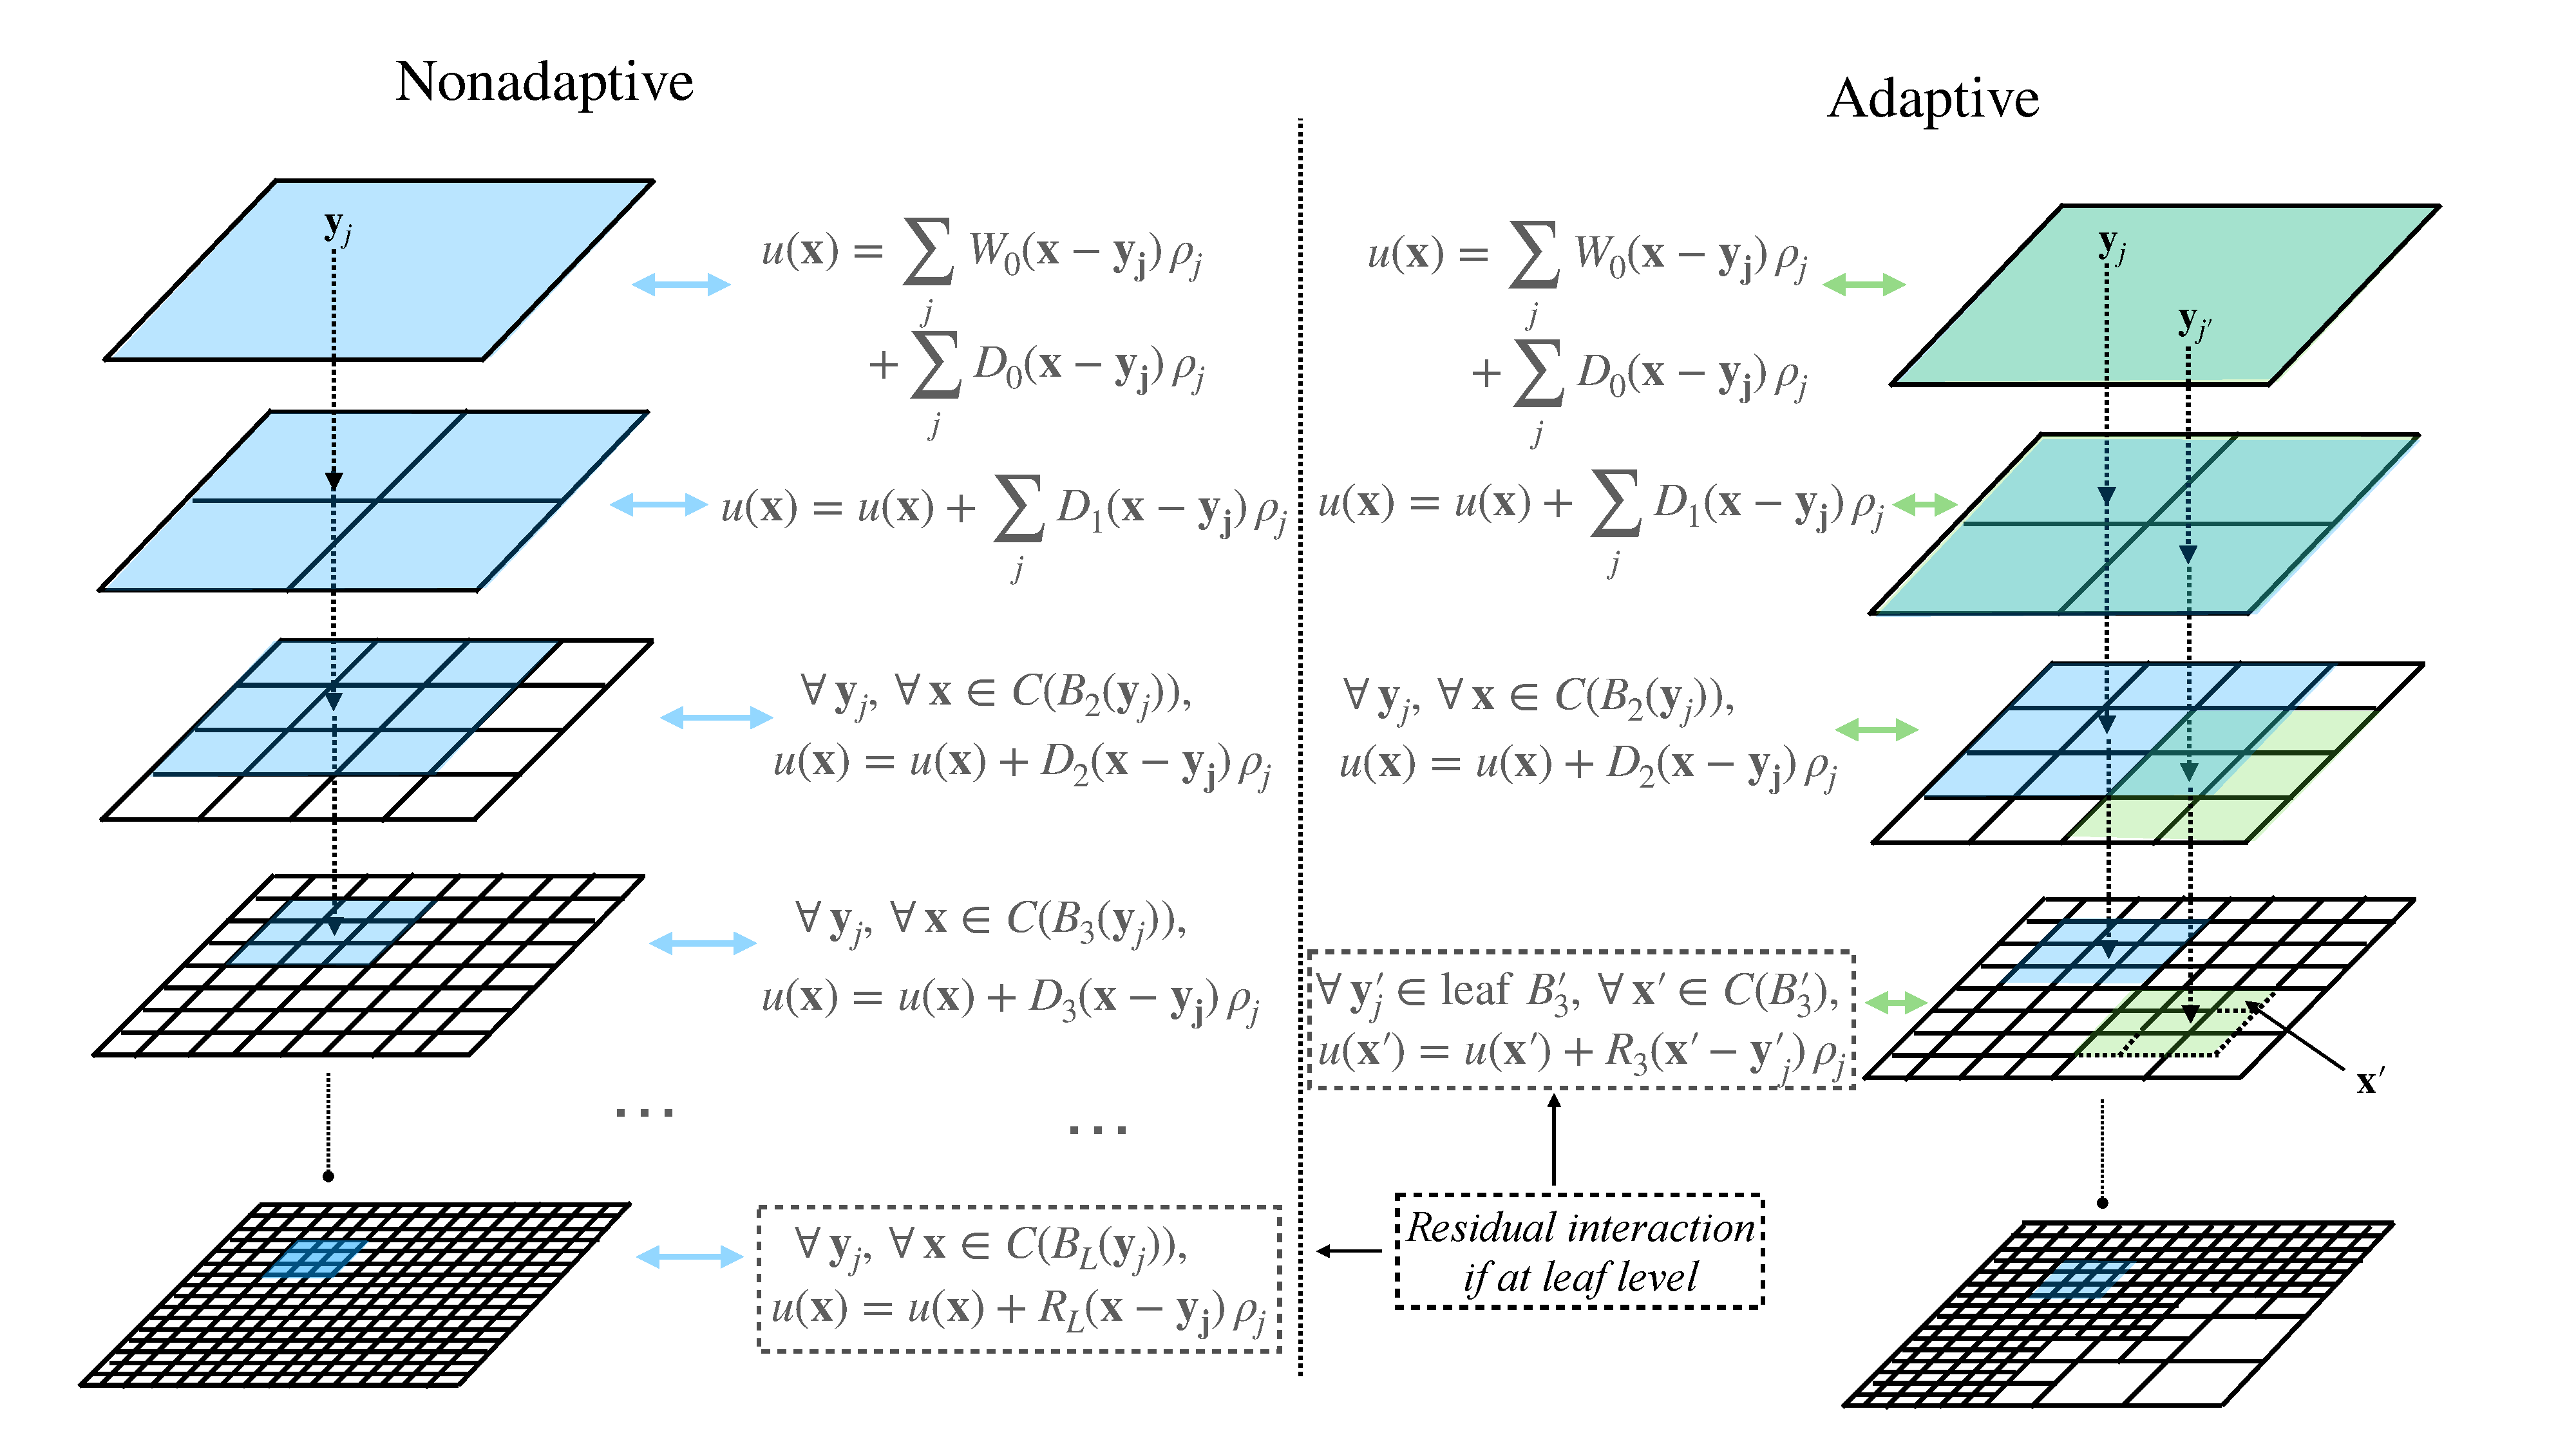
\includegraphics[width=95mm]{dmk_adap.pdf}
\end{center}
{\footnotesize\textsf{In the nonadaptive case (left), each source \(\y_j\) lies in a leaf box \(B\) at the finest level, and the residual kernel \(R_L\) is evaluated over the local colleague boxes. The right panel shows the corresponding adaptive organization.}}
\end{frame}

%----------------------------------------------------------------
\subsection{PSWF kernel splittings}

%================================================================
\begin{frame}{Optimal kernel splitting using prolates}
\small
Let \(r=|\x-\y|\).  With the level length scales \(h_\ell\), the PSWF
construction gives the explicit telescope
\[
  \frac{1}{r}=W_0(r)+\sum_{\ell=0}^{L-1}D_\ell(r)+R_L(r).
\]
\[
\begin{aligned}
  W_0(r)&:=\frac{\Phi_0(r)}{r}, &
  D_\ell(r)&:=\frac{\Phi_{\ell+1}(r)-\Phi_\ell(r)}{r}, &
  R_L(r)&:=\frac{1-\Phi_L(r)}{r},\\[2pt]
  \Phi_\ell(r)&:=\frac{1}{c_0}\int_0^{r/h_\ell}\psi_0^c(t)\dd t, &
  c_0&:=\int_0^1\psi_0^c(t)\dd t, &
  h_{\ell+1}&=h_\ell/2 .
\end{aligned}
\]
\begin{itemize}
  \item \(\psi_0^c\) is the first prolate spheroidal wave function, used as the window at every level.
  \item The difference kernels are smooth and the residual is localized at the finest scale; their Fourier representations remain short at fixed accuracy.
\end{itemize}
{\scriptsize\gray{S.\ Jiang \& L.\ Greengard, \emph{Communications on Pure and Applied Mathematics} 78 (2025).}}
\end{frame}

%================================================================
\begin{frame}{PSWF splitting for the Yukawa kernel}
\footnotesize
For the Yukawa Green's function, let \(k=|\kk|\).  In both two and three
dimensions,
\[
  \widehat G_{\rm Y}(k)=\frac{1}{k^2+\lambda^2}
  =\widehat M_0^c(k)+\sum_{\ell=0}^{L-1}\widehat D_\ell^c(k)+\widehat R_L^c(k).
\]
\[
\begin{aligned}
\widehat M_0^c(k)
  &=\frac{\psi_0^c\!\left(\sqrt{k^2+\lambda^2}\,\cR_0/c\right)}
          {\psi_0^c(0)(k^2+\lambda^2)},\\
\widehat D_\ell^c(k)
  &=\frac{\psi_0^c\!\left(\sqrt{k^2+\lambda^2}\,\cR_{\ell+1}/c\right)
          -\psi_0^c\!\left(\sqrt{k^2+\lambda^2}\,\cR_\ell/c\right)}
          {\psi_0^c(0)(k^2+\lambda^2)},\\
\widehat R_L^c(k)
  &=\frac{1-\psi_0^c\!\left(\sqrt{k^2+\lambda^2}\,\cR_L/c\right)/\psi_0^c(0)}
          {k^2+\lambda^2}.
\end{aligned}
\]
\begin{itemize}\itemsep1pt
  \item Evenness and analyticity of \(\psi_0^c\) make the difference and residual kernels localized in physical space to the requested precision.
  \item The formula is dimension-independent and includes \(\lambda=0\), recovering the Laplace splitting.
\end{itemize}
{\scriptsize\gray{S.\ Jiang \& L.\ Greengard, \emph{Communications on Pure and Applied Mathematics} 78 (2025).}}
\end{frame}

%================================================================
\begin{frame}{A Fourier-space split for \(1/r^2\) in 3D}
\small
\setlength{\abovedisplayskip}{3pt}
\setlength{\belowdisplayskip}{3pt}
The Green's function of \(\sqrt{-\Delta}\) in three dimensions is
\[
  K(r)=\frac{1}{r^2},\qquad \widehat K(\kk)=\frac{2\pi^2}{|\kk|}.
\]
It too admits a PSWF telescope.  With \(\cR_{\ell+1}=\cR_\ell/2\),
\[
  \frac{1}{r^2}=M_0(r)+\sum_{\ell=0}^{L-1}D_\ell(r)+R_L(r),
\]
\[
\begin{aligned}
 M_0(r)&=\frac{1-\psi_0^c(r/\cR_0)/\psi_0^c(0)}{r^2},\\
 D_\ell(r)&=\frac{\psi_0^c(r/\cR_\ell)-\psi_0^c(r/\cR_{\ell+1})}{\psi_0^c(0)r^2},\\
 R_L(r)&=\frac{\psi_0^c(r/\cR_L)}{\psi_0^c(0)r^2}.
\end{aligned}
\]
\begin{itemize}
  \item The relevant Fourier singularity is \(1/|\kk|\), not \(|\kk|\).
\end{itemize}
{\scriptsize\gray{S.\ Jiang \& L.\ Greengard, \emph{Communications on Pure and Applied Mathematics} 78 (2025).}}
\end{frame}

%================================================================
\subsection{Results and synthesis}

\begin{frame}{Performance: point DMK for \(1/r\) in 3D}
\small
\begin{columns}[T,totalwidth=\textwidth]
\begin{column}{0.58\textwidth}
\centering
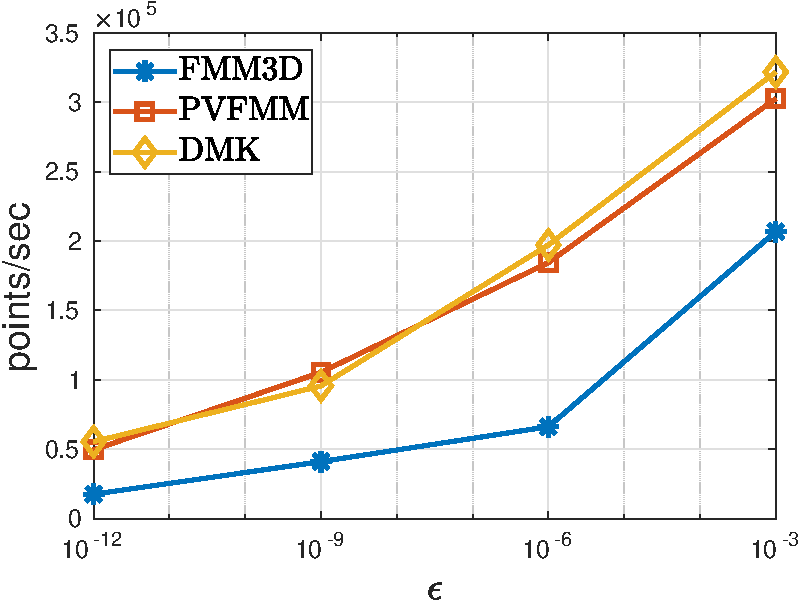
\includegraphics[height=45mm]{l3dpointpps.pdf}
\end{column}
\begin{column}{0.42\textwidth}
\begin{itemize}
  \item Reported benchmark point rate vs.\ requested precision \(\epsilon\).
  \item The reported comparison uses FMM3D and PVFMM as reference implementations.
  \item In these tests, DMK is competitive across the reported accuracies while using the same multilevel organization at every precision.
\end{itemize}
\end{column}
\end{columns}
{\scriptsize\gray{S.\ Jiang \& L.\ Greengard, \emph{Communications on Pure and Applied Mathematics} 78 (2025), Sec.\ 5.1.}}
\end{frame}

%================================================================
\begin{frame}{Performance: box DMK for \(\sqrt{-\Delta}\)}
\small
\begin{columns}[T,totalwidth=\textwidth]
\begin{column}{0.5\textwidth}
\centering
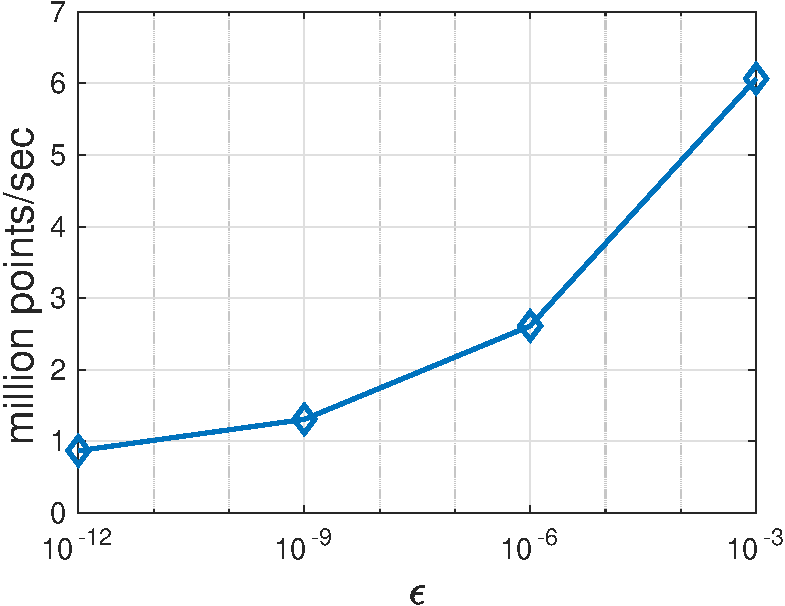
\includegraphics[height=38mm]{sl2dbox.pdf}\\
{\scriptsize 2D}
\end{column}
\begin{column}{0.5\textwidth}
\centering
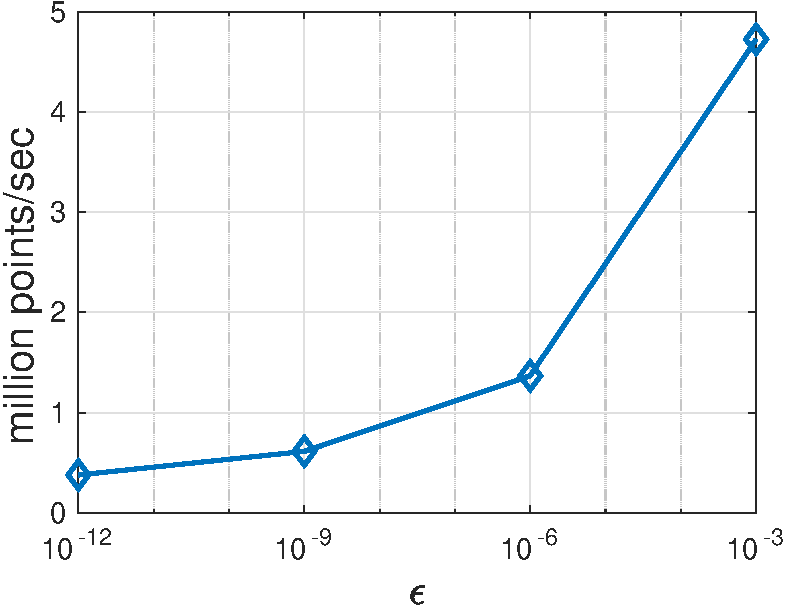
\includegraphics[height=38mm]{sl3dbox.pdf}\\
{\scriptsize 3D}
\end{column}
\end{columns}
\vspace{1mm}
\begin{itemize}
  \item The plots use the Green's functions of \(\sqrt{-\Delta}\): \(1/r\) in 2D and \(1/r^2\) in 3D, up to normalization. Their Fourier transforms are proportional to \(1/|\kk|\), not \(|\kk|\).
  \item These reported box-DMK tests illustrate the framework for kernels beyond the 3D Laplace potential.
\end{itemize}
{\scriptsize\gray{S.\ Jiang \& L.\ Greengard, \emph{Communications on Pure and Applied Mathematics} 78 (2025), Sec.\ 5.1.}}
\end{frame}

%================================================================
\begin{frame}{How DMK combines FMM and Ewald ideas}
\small
\begin{center}
\begin{tabular}{@{}lccc@{}}
\toprule
 & FMM & Fast Ewald & \hl{DMK}\\
\midrule
Complexity & \(\cO(N)\) & \(\cO(N\log N)\) & \(\cO(N)\)\\
Spatial organization & separated tree & uniform mesh & \hl{adaptive tree}\\
Fourier work & none & global FFT & \hl{short sums}\\
Translation & M2L & global multiplier & \hl{diagonal neighbors}\\
Adaptive resolution & yes & no & \hl{yes}\\
\bottomrule
\end{tabular}
\end{center}
\vspace{2mm}
\begin{itemize}
  \item DMK inherits the tree, proxy, and upward/downward organization of the FMM.
  \item It inherits Ewald's Fourier diagonalization, but applies it to short, precision-dependent plane-wave sums at each level rather than one global FFT.
\end{itemize}
{\scriptsize\gray{S.\ Jiang \& L.\ Greengard, \emph{Communications on Pure and Applied Mathematics} 78 (2025).}}
\end{frame}

%================================================================
\begin{frame}{Relation to the FMM and \(\mathcal H\)-matrices}
\small
From a linear-algebra perspective, all methods approximate the dense matrix \(K(\x_i-\y_j)\):
\begin{itemize}
  \item \hl{FMM / \(\mathcal H\)-matrices / skeletonization}: compress the matrix \emph{directly}, block by block; off-diagonal (well-separated) blocks are low rank. Requires near/far separation.
  \item \hl{DMK} (and multilevel summation): write the matrix as a \hl{sum} of matrices, one per scale --- dense but low rank at coarse levels, sparse at fine levels.
  \item DMK's advance over earlier multilevel summation: a \emph{single} convolution kernel per level, diagonalized in Fourier space rather than compressed in physical space.
\end{itemize}
{\scriptsize\gray{S.\ Jiang \& L.\ Greengard, \emph{Communications on Pure and Applied Mathematics} 78 (2025).}}
\end{frame}

%================================================================
\begin{frame}{Precision-dependent parameters for 3D Laplace DMK}
\scriptsize
For the PSWF splitting, the parameters used in the paper are:
\begin{center}
\begin{tabular}{@{}cccccccc@{}}
\toprule
\(\epsilon\) & \(\log(1/\epsilon)\) & \(c\) & \(N_1\) & \(p\) & \(h_0\) & \(N_1^{\rm G}\) & \(p^{\rm G}\) \\
\midrule
\(10^{-3}\)  & \(6.9\)  & \(7.2462\)  & \(13\) & \(9\)  & \(0.6620\pi\) & \(22\) & \(16\) \\
\(10^{-6}\)  & \(13.8\) & \(13.7400\) & \(25\) & \(18\) & \(0.6686\pi\) & \(44\) & \(30\) \\
\(10^{-9}\)  & \(20.7\) & \(20.7360\) & \(39\) & \(28\) & \(0.6625\pi\) & \(66\) & \(46\) \\
\(10^{-12}\) & \(27.6\) & \(27.8700\) & \(53\) & \(38\) & \(0.6677\pi\) & \(88\) & \(62\) \\
\bottomrule
\end{tabular}
\end{center}
\begin{itemize}
  \item \(N_1=2n_f+1\) is the number of Fourier nodes in each dimension; \(p\) is the Chebyshev/proxy-grid order. At level \(l\), \(h_l=2^l h_0\) and \(K_{\max}=2^l c\).
  \item \(N_1^{\rm G}\) and \(p^{\rm G}\) are the corresponding values for the original Gaussian split.
  \item \(n_s\) is selected separately to balance local interactions against the remaining work for the distribution and hardware at hand.
\end{itemize}
{\scriptsize\gray{S.\ Jiang \& L.\ Greengard, \emph{Communications on Pure and Applied Mathematics} 78 (2025), Table 1.}}
\end{frame}

%================================================================
\begin{frame}{DMK connections to later solvers}
\small
\begin{itemize}\itemsep3pt
  \item \hl{Volume potentials / fast Poisson solvers} (Day 4): DMK evaluates \(\int_B G(\x-\y)\rho(\y)\dd\y\) for smooth \(\rho\) --- the ``box DMK''.
  \item \hl{Free-space convolution} (Day 4): a smooth, windowed Fourier kernel is a reusable device for high-order volume-potential evaluation.
  \item \hl{Integral-equation solvers}: when an appropriate DMK split is available, it supplies the fast matrix-vector product in an iterative solver.
\end{itemize}
{\scriptsize\gray{F.\ Vico, L.\ Greengard \& M.\ Ferrando, \emph{Journal of Computational Physics} 323 (2016); S.\ Jiang \& L.\ Greengard, \emph{Communications on Pure and Applied Mathematics} 78 (2025).}}
\end{frame}

%================================================================
\begin{frame}{DMK summary}
\small
\begin{columns}[T,totalwidth=\textwidth]
\begin{column}{0.5\textwidth}
\textbf{The three mechanisms}
\begin{itemize}
  \item \hl{Telescope} the kernel across levels: windowed \(+\) difference \(+\) residual.
  \item \hl{Dual-space}: each piece is evaluated in the lower-cost representation,
  physical or Fourier.
  \item \hl{Diagonal translation}: pure exponentials \(\Rightarrow\) no dense M2L, only neighbors.
\end{itemize}
\end{column}
\begin{column}{0.5\textwidth}
\textbf{Consequence}
\begin{itemize}
  \item Adaptive \(\cO(N)\), global-FFT-free for kernels with an appropriate multilevel split.
  \item The same proxy and diagonal-translation organization can be reused once the kernel-specific split is available.
  \item Unifies the two classical families.
\end{itemize}
\end{column}
\end{columns}
\vspace{5mm}
\begin{center}
\hl{DMK replaces far-field lists by nearest-neighbor interactions on every level
of a multiscale kernel split.}
\end{center}
\end{frame}

%================================================================
\begin{frame}{Morning summary}
\small
\begin{itemize}
  \item \textbf{NUFFT} --- spread, FFT, correct: converts scattered exponential
  sums into FFTs plus localized interpolation work, to any precision.
  \item \textbf{Fast Ewald / ESP} --- one kernel split plus gridding/FFT gives \(\cO(N\log N)\) periodic electrostatics; ESP reduces the required grid at matched tolerance.
  \item \textbf{DMK} --- a hierarchy of kernel splits on an adaptive tree gives \(\cO(N)\) summation and convolution without a global FFT when a suitable kernel split is available.
\end{itemize}
\vspace{2mm}
\begin{block}{The single thread}
Smooth components are evaluated in Fourier space; local components are evaluated in physical space. Choose the split scale(s) to match the data --- once for Ewald, or at every level for DMK.
\end{block}
\vspace{2mm}
\centerline{\gray{This afternoon (M.\ Rachh): the Fast Multipole Method and the high-frequency FMM for Helmholtz.}}
\end{frame}

%================================================================
\begin{frame}{References}
\scriptsize
\begin{itemize}
  \item A.\ Dutt \& V.\ Rokhlin, ``Fast Fourier transforms for nonequispaced data,'' \emph{SIAM Journal on Scientific Computing} 14 (1993).
  \item L.\ Greengard \& J.-Y.\ Lee, ``Accelerating the nonuniform fast Fourier transform,'' \emph{SIAM Review} 46 (2004).
  \item A.\ Barnett, J.\ Magland \& L.\ af Klinteberg, ``A parallel nonuniform FFT library\dots (\texttt{finufft}),'' \emph{SIAM Journal on Scientific Computing} 41 (2019); \texttt{finufft.readthedocs.io}.
  \item P.\ Ewald, ``Die Berechnung optischer und elektrostatischer Gitterpotentiale,'' \emph{Annalen der Physik} 369 (1921); T.\ Darden, D.\ York \& L.\ Pedersen, ``Particle mesh Ewald,'' \emph{Journal of Chemical Physics} 98 (1993); U.\ Essmann et al., ``A smooth particle mesh Ewald method,'' \emph{Journal of Chemical Physics} 103 (1995).
  \item J.\ Liang, L.\ Lu, A.\ Barnett, L.\ Greengard \& S.\ Jiang, ``Accelerating molecular dynamics simulations using fast Ewald summation with prolates,'' \emph{Nature Communications} 17 (2026), doi:10.1038/s41467-026-73232-8.
  \item F.\ Vico, L.\ Greengard \& M.\ Ferrando, ``Fast convolution with free-space Green's functions,'' \emph{Journal of Computational Physics} 323 (2016).
  \item S.\ Jiang \& L.\ Greengard, ``A dual-space multilevel kernel-splitting framework\dots,'' \emph{Communications on Pure and Applied Mathematics} 78 (2025) 1086--1143; \texttt{github.com/flatironinstitute/dmk}.
  \item L.\ Greengard \& V.\ Rokhlin, ``A fast algorithm for particle simulations,'' \emph{Journal of Computational Physics} 73 (1987).
  \item H.\ Cheng, L.\ Greengard \& V.\ Rokhlin, ``A fast adaptive multipole algorithm in three dimensions,'' \emph{Journal of Computational Physics} 155 (1999).
  \item D.\ Osipov, V.\ Rokhlin \& H.\ Xiao, \emph{Prolate Spheroidal Wave Functions of Order Zero}, Springer (2013).
\end{itemize}
\end{frame}

\end{document}
